\documentclass{article}

\usepackage{graphicx}
\usepackage{subcaption}
\usepackage{fancyhdr}
\usepackage[sorting=none]{biblatex}
\usepackage[margin=1in]{geometry}
\usepackage{listings}
\usepackage[hidelinks]{hyperref}
%\usepackage{subfigure}
\usepackage{amsmath}
\usepackage{float}
\usepackage{lmodern} % فونت بهتر برای لاتین
\usepackage{xcolor}
\usepackage{minted}
\usepackage{fvextra}

\setminted{
	linenos,
	breaklines=true,
	breakanywhere=true,
	encoding=utf8,
	autogobble=true,
	fontsize=\small,
	frame=single,
	tabsize=4,
	obeytabs=true,
	mathescape=false,
	texcomments=false
}
\usepackage{amssymb}
\usepackage{longtable} % برای جداول طولانی
\usepackage{enumitem} % برای کنترل لیست‌ها
\usepackage{booktabs} % برای جداول حرفه‌ای
\hypersetup{
	colorlinks=true,
	linkcolor=teal,
	filecolor=magenta,      
	urlcolor=teal,
	citecolor=teal
}
\usepackage{xepersian}




\setlength\headheight{28pt} 
\addbibresource{bibliography.bib}
\settextfont[Path={./font/}, Scale=1.3]{IRLotus}
\setlatintextfont[Scale=1]{Times New Roman}
\renewcommand{\baselinestretch}{1.5}
\pagestyle{fancy}
\fancyhf{}
\lhead{تمرین سری دوم یادگیری ماشین}
\chead{
\includegraphics[width=1cm]{img/Logo.png}}
\rhead{\thepage}

\rfoot{محمدامین محمدیون شبستری}
\cfoot{آرین خوشنویس}
\lfoot{محمدسبحان سخایی}
\renewcommand{\headrulewidth}{1pt}
\renewcommand{\footrulewidth}{1pt}
\AtBeginDocument{
	\def\chapterautorefname{فصل}%
	\def\sectionautorefname{پاسخ سوال}%
	\def\subsectionautorefname{بخش}%
	\def\subsubsectionautorefname{بخش}%
	\def\equationautorefname{رابطهٔ}%
    \def\lstlistingautorefname{برنامۀ}%
}
\renewcommand{\lstlistingname}{Code}

\definecolor{codegreen}{rgb}{0,0.6,0}
\definecolor{codegray}{rgb}{0.5,0.5,0.5}
\definecolor{codepurple}{rgb}{0.58,0,0.82}
\definecolor{backcolour}{rgb}{0.95,0.95,0.92}

\lstdefinestyle{mystyle}{
	backgroundcolor=\color{backcolour},   
	commentstyle=\color{codegreen},
	keywordstyle=\color{magenta},
	numberstyle=\tiny\color{codegray},
	stringstyle=\color{codepurple},
	basicstyle=\ttfamily\footnotesize,
	breakatwhitespace=false,         
	breaklines=true,                 
	captionpos=b,                    
	keepspaces=true,                 
	numbers=left,                    
	numbersep=5pt,                  
	showspaces=false,                
	showstringspaces=false,
	showtabs=false,                  
	tabsize=2
}



\lstset{style=mystyle}

\begin{document}
\begin{titlepage}
\begin{center}
\defpersianfont\nast[Path={./font/}, Scale=1.8]{IranNastaliq}
\centerline{{
\includegraphics[width=4cm]{img/Logo.png}}}
\centerline{\textcolor[rgb]{0,0,0.5}{\nast \bfseries دانشکدۀ مهندسی برق}}

\vspace{0.5cm}

\huge
\textbf{درس یادگیری ماشین}\\[0.4cm]
\textbf{استاد: دکتر امیرحسین نیکوفرد}\\[0.4cm]
\textbf{تمرین سری دوم }\\
\textbf{گروه جاویدنام سپهر ایران }\\
\vspace{1.3cm}

\begin{table}[ht]
\centering
\renewcommand{\arraystretch}{1.35}
\Large
\begin{tabular}{|c|c|}
\hline
نام و نام خانوادگی & محمدامین محمدیون شبستری\\
\hline
شمارهٔ دانشجویی & 40122503\\
\hline
نام و نام خانوادگی & محمدسبحان سخایی\\
\hline
شمارهٔ دانشجویی & 40119253\\
\hline
نام و نام خانوادگی & آرین خوشنویس\\
\hline
شمارهٔ دانشجویی & 40117983\\
\hline

تاریخ & اردیبهشت 1405\\
\hline
%%\multicolumn{2}{|c|}{%
%%\begin{minipage}{0.9\linewidth}
%%\centering
%%\large
%%\textbf{لینک‌های مربوط به کد :}\\[0.3em]
%%\href{https://drive.google.com/file/d/1dC_vEO91lA3BBd1XWn54jxsrS-rq5QCG/view?usp=sharing}
%%{\textcolor{blue}{کد}}
%%\quad | \quad
%%\href{https://github.com/mobinamqdm/fundamentals-of-intelligent-systems-}
%%{\textcolor{blue}{لینک گیت‌هاب}}




%%\end{minipage}}\\
\hline
\end{tabular}
\end{table}

\vfill

\end{center}
\end{titlepage}



\tableofcontents \clearpage
\listoffigures \clearpage
\listoftables \clearpage
\lstlistoflistings \clearpage
\newpage
\section{بخش اول: تحلیل گرادیان و پیاده سازی لایۀ کانولوشن سفارشی(تحت \lr{Pytorch})}
\subsection{استخراج روابط ریاضی دقیق برای گرادیان‌های $\frac{\partial L}{\partial W}$ و $\frac{\partial L}{\partial M}$ با فرض ورودی تک‌کاناله، استراید برابر ۱ و بدون پدینگ $(Padding=0)$}

\subsubsection{روابط کلی حاکم بر سیستم}

فرض کنید ورودی سیستم $X \in \mathbb{R}^{H\times W}$، ماتریس وزن‌های فیلتر $W \in \mathbb{R}^{K\times K}$ و ماتریس ماسک $M \in \mathbb{R}^{K\times K}$ باشد. فیلتر نهایی که روی ورودی اعمال می‌شود حاصل ضرب درایه‌به‌درایه این دو ماتریس است:

\[
W' = W \odot M
\]

که در آن $\odot$ نشان‌دهنده ضرب هادامارد (درایه‌به‌درایه) است.

با فرض یک ورودی تک‌کاناله، استراید برابر ۱ و بدون پدینگ $(Padding = 0)$، خروجی لایه کانولوشن برابر است با کانولوشن ورودی با فیلتر نهایی:

\[
Y = X * W'
\]

اگر ابعاد فیلتر $K\times K$ باشد، آنگاه با بسط رابطه کانولوشن در سطح درایه‌ها داریم:

\[
y_{i,j} =
\sum_{m=0}^{K-1}
\sum_{n=0}^{K-1}
X_{i+m,j+n} \, W'_{m,n}
\]

با جایگذاری $W' = W \odot M$ خواهیم داشت:

\[
y_{i,j} =
\sum_{m=0}^{K-1}
\sum_{n=0}^{K-1}
X_{i+m,j+n}\,(W_{m,n}M_{m,n})
\]

که در آن $i,j$ اندیس‌های موقعیت در خروجی هستند.

تابع خطای مورد استفاده در این مسئله میانگین مربعات خطا \lr{(Mean Squared Error)} است که به صورت زیر تعریف می‌شود:

\[
L =
\frac{1}{N}
\sum_{i}\sum_{j}
(Y_{i,j}-\hat{Y}_{i,j})^2
\]

که در آن $\hat{Y}$ خروجی هدف (Target) و $N$ تعداد کل عناصر خروجی است.

\subsubsection{محاسبه گرادیان ماتریس‌های وزن و ماسک مدل}

برای محاسبه گرادیان‌ها از قاعده زنجیره‌ای استفاده می‌کنیم.

ابتدا مشتق تابع خطا نسبت به خروجی شبکه محاسبه می‌شود:

\[
\frac{\partial L}{\partial Y_{i,j}}
=
\frac{2}{N}(Y_{i,j}-\hat{Y}_{i,j})
\]

اکنون گرادیان نسبت به وزن‌های فیلتر را محاسبه می‌کنیم. با استفاده از قاعده زنجیره‌ای داریم:

\[
\frac{\partial L}{\partial W_{m,n}}
=
\sum_i \sum_j
\frac{\partial L}{\partial Y_{i,j}}
\frac{\partial Y_{i,j}}{\partial W_{m,n}}
\]

با توجه به رابطه تعریف شده برای $y_{i,j}$ داریم:

\[
Y_{i,j} =
\sum_{m=0}^{K-1}\sum_{n=0}^{K-1}
X_{i+m,j+n}(W_{m,n}M_{m,n})
\]

بنابراین مشتق آن نسبت به $W_{m,n}$ برابر است با:

\[
\frac{\partial Y_{i,j}}{\partial W_{m,n}}
=
X_{i+m,j+n}\,M_{m,n}
\]

در نتیجه گرادیان وزن‌ها به صورت زیر به دست می‌آید:

\[
\frac{\partial L}{\partial W_{m,n}}
=
\sum_i \sum_j
\frac{\partial L}{\partial Y_{i,j}}
\,
X_{i+m,j+n}
\,M_{m,n}
\]

که می‌توان آن را به صورت زیر بازنویسی کرد:

\[
\frac{\partial L}{\partial W_{m,n}}
=
M_{m,n}
\sum_i \sum_j
\frac{\partial L}{\partial Y_{i,j}}
X_{i+m,j+n}
\]

به طور مشابه گرادیان نسبت به ماسک نیز از قاعده زنجیره‌ای به دست می‌آید:

\[
\frac{\partial L}{\partial M_{m,n}}
=
\sum_i \sum_j
\frac{\partial L}{\partial Y_{i,j}}
\frac{\partial Y_{i,j}}{\partial M_{m,n}}
\]

از رابطه خروجی داریم:

\[
\frac{\partial Y_{i,j}}{\partial M_{m,n}}
=
X_{i+m,j+n}\,W_{m,n}
\]

بنابراین:

\[
\frac{\partial L}{\partial M_{m,n}}
=
W_{m,n}
\sum_i \sum_j
\frac{\partial L}{\partial Y_{i,j}}
X_{i+m,j+n}
\]

در نهایت می‌توان روابط گرادیان‌ها را به صورت فشرده در قالب عملیات ماتریسی نوشت. اگر

\[
\delta = \frac{\partial L}{\partial Y}
\]

را گرادیان خطا نسبت به خروجی در نظر بگیریم، آنگاه خواهیم داشت:

\[
\frac{\partial L}{\partial W}
=
M \odot (X \star \delta)
\]

\[
\frac{\partial L}{\partial M}
=
W \odot (X \star \delta)
\]

که در آن $\star$ نشان‌دهنده عملیات \lr{cross-correlation} بین ورودی و گرادیان خروجی است.

بنابراین گرادیان وزن‌ها و ماسک‌ها هر دو به کانولوشن ورودی با گرادیان خروجی وابسته هستند و تنها تفاوت آن‌ها در ضریب درایه‌ای $M$ و $W$ است.
\subsection{پیاده‌سازی لایۀ سیستم با استفاده از عملیات \lr{Unfold} در PyTorch}

در این بخش، لایه کانولوشنی که روابط ریاضی آن در قسمت قبل استخراج شد، با استفاده از عملیات \lr{unfold} از کتابخانه‌ی PyTorch پیاده‌سازی می‌شود. در این پیاده‌سازی، از ماژول \lr{nn.Conv2d} استفاده نشده و عملیات کانولوشن به صورت دستی و مبتنی بر ضرب ماتریسی بین پچ‌های ورودی و فیلتر نهایی انجام می‌گیرد.

\subsubsection{ایجاد داده‌های ورودی و پارامترهای مدل}

به منظور آزمایش عملکرد لایه و بررسی گرادیان‌ها، یک \lr{Tensor} ورودی تصادفی با ابعاد $(1,1,5,5)$ و یک \lr{Tensor} هدف با ابعاد $(1,1,3,3)$ ساخته می‌شود. دو پارامتر قابل آموزش به نام‌های $W$ و $M$ با ابعاد $3\times3$ برای وزن‌های فیلتر و ماسک تعریف شده‌اند. همان‌گونه که در بخش روابط ریاضی گفته شد، فیلتر نهایی برابر است با ضرب درایه‌به‌درایه دو ماتریس مذکور:

\[
W' = W \odot M
\]

که در آن $\odot$ نشان‌دهنده‌ی ضرب هادامارد یا ضرب درایه‌ای است.

\subsubsection{پیاده‌سازی عملیات کانولوشن با استفاده از \lr{unfold}}

تابع \lr{torch.nn.functional.unfold} یک عملیات پایه‌ای در PyTorch است که وظیفه‌ی آن استخراج تمام پنجره‌های متوالی (پچ‌ها) از تصویر ورودی است.  
برای یک ورودی $5\times5$ و فیلتر با اندازه‌ی هسته‌ی $3\times3$، تابع \lr{unfold} تمامی زیرفرم‌های $3\times3$ را بدون همپوشانی استخراج کرده و آن‌ها را در قالب یک ماتریس با ابعاد $(9,9)$ قرار می‌دهد (در این مثال ۹ پچ وجود دارد، هر پچ شامل ۹ درایه است).

در ادامه، ماتریس وزن نهایی $W'$ تخت (Flatten) شده و در قالب یک بردار ردیفی با طول $9$ قرار می‌گیرد. عملیات کانولوشن معادل ضرب ماتریسی بین این بردار و ماتریس پچ‌ها است و حاصل آن همان خروجی لایه کانولوشنی خواهد بود:

\[
output\_flat = W'_{flat} \times patches
\]

سپس این خروجی دوباره به ابعاد اصلی کانولوشن یعنی $(1,1,3,3)$ تغییر شکل داده می‌شود.

\subsubsection{محاسبه تابع خطا و انجام عملیات \lr{Backpropagation}}

در گام بعد، تابع خطای میانگین مربعات خطا \lr{(MSE)} بین خروجی شبکه و مقدار هدف محاسبه می‌شود:

\[
L = \frac{1}{N} \sum_i \sum_j (Y_{i,j} - \hat{Y}_{i,j})^2
\]

با استفاده از تابع \lr{criterion = nn.MSELoss()} در \LR{PyTorch}، مقدار خطا محاسبه شده و سپس با فراخوانی \lr{loss.backward()} مشتقات یا گرادیان‌های پارامترهای مدل به دست می‌آیند.  
در فرآیند آموزش، این گرادیان‌ها برای بروزرسانی پارامترهای $W$ و $M$ به کار خواهند رفت.

\subsubsection{کد}
\begin{LTR}
	\inputminted{python}{code/ml_hw2_q1.py}
\end{LTR}

\subsubsection{نتایج اجرای برنامه}

پس از اجرای یک مرحله‌ی \lr{Forward} و سپس \lr{Backward}، مقدار تابع خطا و گرادیان‌های پارامترهای مدل به صورت نمونه زیر به دست آمده است:

\[
Loss = 4.6200
\]

\[
\nabla_W =
\begin{bmatrix}
	1.1261 & -1.0485 & 0.1057 \\
	2.9304 & 4.1833 & 0.9999 \\
	0.8946 & -0.9351 & -1.2069
\end{bmatrix}
\]

\[
\nabla_M =
\begin{bmatrix}
	0.4340 & -0.3002 & -1.0274 \\
	2.1227 & 2.5464 & -1.0235 \\
	-0.9933 & 0.2171 & -6.0293
\end{bmatrix}
\]

\subsubsection{تحلیل و بررسی نتایج}

همان‌گونه که مشاهده می‌شود، مقدار گرادیان‌های حاصل برای پارامترهای $W$ و $M$ همگی مقادیر عددی غیرصفر هستند.  
این موضوع نشان می‌دهد که مدل به درستی توانسته است جریان گرادیان را از خروجی به پارامترها منتقل کرده و فرآیند \lr{backpropagation} بدون مشکل اجرا شده است.

از آنجا که تابع خطا \lr{MSE} نسبت به پارامترهای مدل مشتق‌پذیر است، در هر مرحله‌ی آموزش وزن‌ها و ماسک‌ها با استفاده از این گرادیان‌ها به روز خواهند شد. این نتیجه تأیید می‌کند که پیاده‌سازی لایه کانولوشن با استفاده از عملیات \lr{unfold} در PyTorch از نظر ریاضی و الگوریتمی سازگار است و رفتار آن با مدل‌های استاندارد \lr{Conv2d} هم‌خوانی دارد.
\newpage

\section{بخش دوم : معماری \lr{Bottleneck} در \lr{Resnet} و مدیریت منابع محاسباتی}
\subsection{محاسبه تحلیلی تعداد پارامترهای بلوک \lr{Bottleneck} در \lr{ResNet}}

در معماری \lr{ResNet}، بلوک‌های \lr{Bottleneck} برای کاهش بار محاسباتی و در عین حال حفظ توان نمایش مدل به کار می‌روند. ایده اصلی این بلوک‌ها آن است که ابتدا با یک کانولوشن \(1\times1\) تعداد کانال‌ها کاهش یابد، سپس پردازش فضایی با کانولوشن \(3\times3\) روی نمایش فشرده‌تر انجام شود، و در نهایت با یک کانولوشن \(1\times1\) تعداد کانال‌ها دوباره به مقدار اولیه بازگردد.

در این مسئله، ورودی بلوک دارای ابعاد زیر است:

\[
(Batch=1,\; Channels=256,\; H=14,\; W=14)
\]

ساختار بلوک نیز شامل سه لایه کانولوشنی متوالی به صورت زیر است:

\[
1\times1 \; (64), \qquad 3\times3 \; (64), \qquad 1\times1 \; (256)
\]

فرض می‌کنیم در هیچ‌یک از لایه‌ها از \lr{Bias} و \lr{Batch Normalization} استفاده نشده است.

\subsubsection{فرمول کلی تعداد پارامترها در کانولوشن}

تعداد پارامترهای یک لایه کانولوشن دوبعدی بدون \lr{Bias} از رابطه زیر به دست می‌آید:

\[
\text{Parameters} = K_h \times K_w \times C_{in} \times C_{out}
\]

که در آن:
\begin{itemize}
	\item \(K_h\) و \(K_w\) به ترتیب ارتفاع و عرض هسته کانولوشن هستند،
	\item \(C_{in}\) تعداد کانال‌های ورودی است،
	\item \(C_{out}\) تعداد فیلترها یا کانال‌های خروجی است.
\end{itemize}

\paragraph{نکته}
ابعاد فضایی ورودی یعنی \(14\times14\) و همچنین اندازه بچ برابر با 1، در تعداد پارامترهای قابل یادگیری تأثیری ندارند و فقط بر حجم محاسبات و ابعاد خروجی لایه‌ها اثر می‌گذارند.

\subsubsection{محاسبه پارامترهای هر لایه}

\paragraph{لایه اول: کانولوشن \(1\times1\)}
این لایه برای کاهش تعداد کانال‌ها از 256 به 64 استفاده می‌شود. بنابراین:

\[
\text{Parameters}_1 = 1 \times 1 \times 256 \times 64 = 16384
\]

\paragraph{لایه دوم: کانولوشن \(3\times3\)}
ورودی این لایه خروجی لایه قبل است، بنابراین تعداد کانال‌های ورودی 64 خواهد بود. در نتیجه:

\[
\text{Parameters}_2 = 3 \times 3 \times 64 \times 64 = 36864
\]

\paragraph{لایه سوم: کانولوشن \(1\times1\)}
این لایه تعداد کانال‌ها را از 64 به 256 بازمی‌گرداند. بنابراین:

\[
\text{Parameters}_3 = 1 \times 1 \times 64 \times 256 = 16384
\]

\subsubsection{تعداد کل پارامترهای بلوک}

با جمع تعداد پارامترهای سه لایه، تعداد کل پارامترهای قابل یادگیری بلوک \lr{Bottleneck} برابر خواهد بود با:

\[
\text{Total Parameters}
= 16384 + 36864 + 16384
= 69632
\]

بنابراین، تعداد دقیق پارامترهای این بلوک برابر است با:

\[
\boxed{69632}
\]
\subsection{کاهش تعداد پارامترهای بلوک \lr{Bottleneck} برای اجرای مدل روی دستگاه‌های لبه}

در کاربردهایی که مدل باید روی دستگاه‌های لبه (\lr{Edge Device}) با محدودیت شدید حافظه اجرا شود، کاهش تعداد پارامترهای مدل اهمیت زیادی دارد. یکی از روش‌های رایج برای کاهش پیچیدگی مدل، کاهش تعداد فیلترهای میانی در بلوک \lr{Bottleneck} است.

در اینجا تعداد فیلترهای میانی از \(64\) به \(32\) کاهش داده می‌شود. در نتیجه، تعداد پارامترهای هر لایه مجدداً محاسبه می‌شود.

\subsubsection{محاسبه تعداد پارامترهای ساختار جدید}

\paragraph{لایه اول: کانولوشن \(1\times1\)}

این لایه تعداد کانال‌ها را از \(256\) به \(32\) کاهش می‌دهد. بنابراین تعداد پارامترها برابر است با:

\[
1 \times 1 \times 256 \times 32 = 8192
\]

\paragraph{لایه دوم: کانولوشن \(3\times3\)}

در این لایه ورودی و خروجی هر دو دارای \(32\) کانال هستند. بنابراین:

\[
3 \times 3 \times 32 \times 32 = 9216
\]

\paragraph{لایه سوم: کانولوشن \(1\times1\)}

این لایه تعداد کانال‌ها را از \(32\) به \(256\) افزایش می‌دهد. بنابراین:

\[
1 \times 1 \times 32 \times 256 = 8192
\]

\subsubsection{تعداد کل پارامترهای بلوک اصلاح شده}

با جمع تعداد پارامترهای سه لایه خواهیم داشت:

\[
8192 + 9216 + 8192 = 25600
\]

در حالت اولیه، تعداد کل پارامترهای بلوک برابر با:

\[
69632
\]

بود. بنابراین درصد کاهش پارامترها برابر است با:

\[
\frac{69632 - 25600}{69632} \times 100
\]

\[
= 63.24\%
\]

در نتیجه با کاهش تعداد فیلترهای میانی از \(64\) به \(32\)، تعداد پارامترهای این بلوک بیش از \(63\%\) کاهش می‌یابد که برای اجرای مدل روی دستگاه‌های لبه با محدودیت حافظه بسیار مفید است.

\subsubsection{تأثیر بر میدان دریافت (\lr{Receptive Field})}

کاهش تعداد فیلترهای میانی هیچ تأثیری بر میدان دریافت ندارد. میدان دریافت تنها به عواملی مانند اندازه فیلترها، مقدار \lr{stride} بستگی دارد.

از آنجا که اندازه فیلترها (\(1\times1\) و \(3\times3\)) و مقدار \lr{stride} در این بلوک تغییری نکرده‌اند، هر نورون در خروجی بلوک همچنان همان ناحیه از تصویر ورودی را مشاهده می‌کند که در حالت اولیه مشاهده می‌کرد.

\subsubsection{تأثیر بر ظرفیت استخراج ویژگی}

کاهش تعداد فیلترها از \(64\) به \(32\) باعث کاهش ظرفیت استخراج ویژگی مدل می‌شود.

\paragraph{کاهش پهنای شبکه}

با نصف شدن تعداد فیلترها، تعداد نگاشت‌های ویژگی (\lr{Feature Maps}) نیز کاهش می‌یابد و در نتیجه تعداد الگوهای متفاوتی که لایه \(3\times3\) می‌تواند شناسایی کند کمتر خواهد شد.

\paragraph{ایجاد گلوگاه قوی‌تر}

کاهش تعداد کانال‌های میانی باعث ایجاد یک \lr{Bottleneck} شدیدتر در مسیر عبور اطلاعات می‌شود. این موضوع می‌تواند باعث کاهش توان مدل در یادگیری ویژگی‌های پیچیده شود.

در مجموع، این تغییر باعث می‌شود مدل سبک‌تر و سریع‌تر اجرا شود که برای دستگاه‌های لبه بسیار مناسب است، اما ممکن است در برخی مسائل باعث کاهش جزئی در دقت مدل شود، در حالی که میدان دریافت شبکه بدون تغییر باقی می‌ماند.
\subsection{پیاده‌سازی و بررسی تجربی بلوک \lr{Bottleneck} در \lr{PyTorch}}

به منظور بررسی درستی محاسبات تحلیلی انجام شده در بخش‌های قبل، دو نسخه از بلوک \lr{Bottleneck} با استفاده از کتابخانه \lr{PyTorch} پیاده‌سازی شد. در نسخه اول تعداد فیلترهای میانی برابر با \(64\) و در نسخه دوم برابر با \(32\) در نظر گرفته شده است. در هر دو مدل از سه لایه کانولوشنی متوالی زیر استفاده شده است:

\[
1\times1 \rightarrow 3\times3 \rightarrow 1\times1
\]

در این پیاده‌سازی از ماژول \lr{nn.Conv2d} استفاده شده و مطابق با فرض مسئله، هیچ \lr{Bias}ای در لایه‌ها در نظر گرفته نشده است.

\subsubsection{پیاده‌سازی بلوک در \lr{PyTorch}}

در ابتدا یک کلاس به نام \lr{BottleneckBlock} تعریف می‌شود که ساختار کامل بلوک را شامل می‌شود. این کلاس سه لایه کانولوشنی را ایجاد کرده و در تابع \lr{forward} ورودی را به صورت متوالی از این لایه‌ها عبور می‌دهد.
\subsubsection{کد}
\begin{LTR}
	\inputminted{python}{code/ml_hw2_q2.py}
\end{LTR}


\paragraph{توضیحات کد}

در ادامه وظیفه هر بخش از کد توضیح داده شده است:

\begin{itemize}
	\item \textbf{فراخوانی کتابخانه‌ها}:  
	با استفاده از \texttt{torch} و \texttt{torch.nn} امکان تعریف شبکه‌های عصبی و لایه‌های کانولوشن فراهم می‌شود.
	
	\item \textbf{تعریف کلاس \lr{BottleneckBlock}}:  
	این کلاس از \lr{nn.Module} ارث‌بری کرده و سه لایه کانولوشنی را مطابق ساختار بلوک‌های Bottleneck پیاده‌سازی می‌کند.
	
	\item \textbf{لایه اول}:  
	کانولوشن \(1\times1\) برای کاهش تعداد کانال‌ها از \lr{in\_channels} به \lr{mid\_channels}.  
	\[
	1\times1\times \text{in\_channels} \times \text{mid\_channels}
	\]
	
	\item \textbf{لایه دوم}:  
	کانولوشن \(3\times3\) با \lr{padding=1} برای حفظ ابعاد فضایی.  
	\[
	3\times3\times \text{mid\_channels}^2
	\]
	
	\item \textbf{لایه سوم}:  
	کانولوشن \(1\times1\) برای بازگرداندن تعداد کانال‌ها به \lr{out\_channels}.  
	\[
	1\times1\times \text{mid\_channels} \times \text{out\_channels}
	\]
	
	\item \textbf{تابع \lr{forward}}:  
	ورودی به ترتیب از سه لایه عبور می‌کند. هدف تنها بررسی ساختار و محاسبه تعداد پارامترها است، بنابراین تابع فعال‌سازی حذف شده است.
	
	\item \textbf{ورودی تصادفی}:  
	تنسوری با ابعاد استاندارد:
	\[
	(1, 256, 14, 14)
	\]
	
	\item \textbf{ساخت مدل 64 فیلتر}:  
	تعداد پارامترها با \texttt{numel()} محاسبه شده و خروجی مدل ذخیره می‌شود.
	
	\item \textbf{ساخت مدل 32 فیلتر}:  
	مشابه مدل اول اما تعداد فیلترهای میانی نصف شده است، بنابراین انتظار کاهش چشمگیر پارامترها وجود دارد.
	
	\item \textbf{چاپ خروجی}:  
	شامل تعداد کل پارامترها و شکل خروجی هر مدل جهت مقایسه با محاسبات تحلیلی.
\end{itemize}

\subsubsection{نتایج اجرای برنامه}

پس از اجرای کد، خروجی زیر به دست می‌آید:

\begin{latin}
	\begin{verbatim}
		Model with 64 filters
		---------------------
		Total Parameters : 69632
		Output Shape     : torch.Size([1, 256, 14, 14])
		
		Model with 32 filters
		---------------------
		Total Parameters : 25600
		Output Shape     : torch.Size([1, 256, 14, 14])
	\end{verbatim}
\end{latin}


\subsubsection{تحلیل نتایج}

\paragraph{تطابق تعداد پارامترها}

خروجی کد نشان می‌دهد که تعداد پارامترهای محاسبه‌شده دقیقاً با محاسبات نظری بخش‌های قبل مطابقت دارد:

\[
69632 \quad \text{:برای مدل با 64 فیلتر}
\]

\[
25600 \quad \text{:برای مدل با 32 فیلتر}
\]

این مطابقت نشان‌دهنده درستی کامل پیاده‌سازی و تحلیل است.

\paragraph{ثابت بودن ابعاد خروجی}

در هر دو مدل ابعاد خروجی یکسان است:

\[
(1, 256, 14, 14)
\]

این نتیجه به دلیل موارد زیر است:
\begin{itemize}
	\item تعداد کانال‌های خروجی در هر دو مدل برابر با 256 تنظیم شده است.
	\item در لایه \(3\times3\) از \lr{padding=1} استفاده شده است که باعث حفظ ابعاد فضایی می‌شود.
\end{itemize}

در نتیجه، کاهش فیلترهای میانی تنها باعث کاهش تعداد پارامترها می‌شود و هیچ تأثیری بر ابعاد خروجی بلوک ندارد.
`
\newpage


\section{بخش سوم: معماری \lr{YOLO} و ترکیب با معیار \lr{Soft Dice Score}}

\subsection{طراحی تابع خطای YOLO مبتنی بر \lr{Soft Dice Score} برای بهبود مکان‌یابی}

\subsubsection{مقدمه}
مدل YOLO یک رگرسور یکپارچه برای تشخیص شیء است که تصویر را به شبکه‌ای $S \times S$ تقسیم کرده و در هر سلول، $B$ جعبه مرزی \lr{(Bounding box)}، مقدار اعتماد \lr{(Confidence)} و توزیع احتمال کلاس‌ها را پیش‌بینی می‌کند. بخش مهم این معماری، \textbf{مکان‌یابی} است که تعیین می‌کند مدل چقدر دقیق مختصات و اندازهٔ جعبه را یاد گرفته است.

در YOLO کلاسیک این بخش با تابع خطای MSE انجام می‌شود؛ تابعی که به دلیل وابستگی شدید به مقیاس اشیاء، در مواجهه با اشیای کوچک عملکرد ضعیفی دارد. در این نوشتار یک تابع خطای جدید مبتنی بر \lr{Soft Dice Score} معرفی می‌کنیم که رفتار کاملاً نرمال‌شده داشته و کیفیت همپوشانی هندسی جعبه‌ها را مستقیماً آموزش می‌دهد.

\subsubsection{محدودیت‌های MSE در مکان‌یابی}
تابع مکان‌یابی YOLO به صورت زیر است:

$$
\begin{aligned}
	L_{loc}^{MSE} =
	\lambda_{coord} 
	\sum_{i=0}^{S^2} \sum_{j=0}^{B} 
	\mathbb{1}_{ij}^{obj}
	\left[
	(x_i - \hat{x}_i)^2 +
	(y_i - \hat{y}_i)^2 +
	(\sqrt{w_i} - \sqrt{\hat{w}_i})^2 +
	(\sqrt{h_i} - \sqrt{\hat{h}_i})^2
	\right]
\end{aligned}
$$

\textbf{مشکل اصلی:}  
MSE برای اشیای کوچک به‌شدت حساس است، زیرا همان جابه‌جایی چندپیکسلی که برای یک شیء بزرگ ناچیز است، برای شیء کوچک منجر به از دست رفتن کامل همپوشانی می‌شود. اما مدل در هر دو حالت یک جریمه مشابه دریافت می‌کند.

این سبب می‌شود \lr{YOLO}:
\begin{itemize}
	\item در آموزش روی اشیای کوچک ضعیف‌تر عمل کند،
	\item گرادیان‌های نامرتبط با همپوشانی دریافت کند
	\item و هماهنگی ضعیفی با معیارهای IoU و همپوشانی واقعی داشته باشد.
\end{itemize}

\subsubsection{تعریف \lr{Soft Dice Score} برای \lr{Bounding Box}}
معیار Dice برای دو ناحیه $A$ و $B$:

$$
Dice(A,B) = \frac{2|A\cap B|}{|A| + |B|}
$$

و نسخه‌ی قابل استفاده در یادگیری:

$$
L_{DiceBox} = 1 - \frac{2I + \epsilon}{A_{gt} + A_p + \epsilon}
$$

که در آن $I$ مساحت همپوشانی و $A_{gt}, A_p$ مساحت جعبه‌ها هستند. این تابع:
\begin{itemize}
	\item کاملاً نرمال‌شده است،
	\item وابسته به همپوشانی واقعی است
	\item و نسبت به مقیاس اشیاء پایدار است.
\end{itemize}

\paragraph{چرا $\epsilon$ ضروری است؟ (تحلیل ریاضی و رفتاری)}
وجود $\epsilon$ حیاتی است، چون:

\begin{enumerate}
	\item \textbf{برای جلوگیری از تقسیم بر صفر}
	
	اگر در ابتدای آموزش، مدل جعبه‌ای بدون مساحت یا کاملاً اشتباه پیش‌بینی کند، یعنی:
	$$ A_p = 0,\qquad I = 0 $$
	
	آن‌گاه مخرج بدون $\epsilon$ می‌شود:
	$$ A_{gt} + A_p = A_{gt} $$
	
	و اگر $A_{gt}=0$ یا جعبهٔ صفر باشد، مخرج صفر شده و مقدار:
	$$ \frac{2I}{A_{gt}+A_p} $$
	تعریف‌نشده است. وجود $\epsilon$ باعث می‌شود که این حالات مشکلی ایجاد نکنند.
	
	\item \textbf{برای پایدار کردن گرادیان هنگام همپوشانی صفر}
	
	اگر هیچ همپوشانی وجود نداشته باشد:
	$$ I=0 $$
	آنگاه بدون $\epsilon$ داریم:
	$$ L = 1 $$
	اما گرادیان‌ها بسیار تیز (Sharp) و ناپایدار می‌شوند. اضافه کردن $\epsilon$ باعث می‌شود صورت کاملاً صفر نشود:
	$$ 2I + \epsilon = \epsilon $$
	و تابع کاملاً شناور و نرم باقی بماند.
	
	\item \textbf{برای جلوگیری از جهش ناگهانی Loss هنگام تماس نقطه‌ای}
	
	اگر دو جعبه فقط یک تماس کوچک یا ۱ پیکسل همپوشانی داشته باشند:
	$$ I \approx 1 $$
	تغییر از $I=0$ به $I=1$ باعث یک پرش بسیار بزرگ در مقدار Loss می‌شود. وجود $\epsilon$ این پرش را تعدیل و هموار می‌کند.
	
	\item \textbf{برای هماهنگی با معیارهای پیوسته در شبکه‌های عصبی}
	
	توابع یادگیری مانند Dice Loss باید مشتق‌پذیر و نرم باشند. اما حالت‌های:
	$$ A_{gt}=0,\quad A_p=0,\quad I=0 $$
	سه نقطهٔ تکین (Singular) هستند. اضافه کردن $\epsilon$ این نقاط را صاف (Smooth) می‌کند.
\end{enumerate}

به طور خلاصه:
$$ \epsilon \text{ برای جلوگیری از ناپایداری عددی و گرادیان لازم است.} $$

\subsubsection{مثال‌های عددی}

\paragraph{مثال عددی با تابع خطای \lr{Soft Dice score}}
\begin{itemize}
	\item $B_{gt}$ مرکز $(25,25)$، عرض $8$، ارتفاع $6$
	\item $B_p$ مرکز $(28,26)$، عرض $8$، ارتفاع $6$
	\item مقدار $\epsilon = 10^{-6}$
\end{itemize}

\textbf{گام ۱: تبدیل مرکز به گوشه‌ها}
$$ B_{gt}: (21,22,29,28) $$
$$ B_{p}: (24,23,32,29) $$

\textbf{گام ۲: محاسبهٔ همپوشانی}
$$ x_{int1}=max(24,21)=24,\quad x_{int2}=min(29,32)=29,\quad w_{int}=29-24=5 $$
$$ y_{int1}=max(22,23)=23,\quad y_{int2}=min(28,29)=28,\quad h_{int}=28-23=5 $$
$$ I = 5 \times 5 = 25 $$

\textbf{گام ۳: مساحت‌ها}
$$ A_{gt}=8 \times 6 = 48,\qquad A_p =8 \times 6 = 48 $$

\textbf{گام ۴: محاسبۀ \lr{Soft Dice Score}}
$$ Soft Dice Score = \frac{2I + \epsilon}{A_{gt} + A_p + \epsilon} = \frac{50 + 10^{-6}}{96 + 10^{-6}} $$
چون مقدار $\epsilon$ بسیار کوچک است، مقدار نهایی تفاوت اندکی دارد:
$$ Dice \approx 0.520833 $$

\textbf{گام ۵: \lr{Dice Loss}}
$$ L_{DiceBox} = 1 - Dice \approx 1 - 0.520833 = 0.479167 $$

\paragraph{مثال عددی با تابع خطای \lr{MSE}}
در همین مثال، اختلاف مراکز:
$$ |x-\hat{x}|=|25-28|=3,\qquad |y-\hat{y}|=|26-25|=1 $$
اگر صرفاً از MSE استفاده شود:
$$ MSE_{xy} = 3^2 + 1^2 = 10 $$

نکتهٔ مهم:
\begin{itemize}
	\item با وجود خطای 3 پیکسلی، جعبهٔ پیش‌بینی هنوز همپوشانی \textbf{۵۰٪} دارد و تشخیص کاملاً قابل قبول است.
	\item ولی MSE این خطا را مانند یک خطای کاملاً بد جریمه می‌کند.
	\item DiceLoss مستقیماً کیفیت همپوشانی را اندازه‌گیری می‌کند.
\end{itemize}

\subsubsection{فرمول نهایی تابع خطای YOLO-Dice}
$$
\begin{aligned}
	L_{YOLO-Dice} =
	\sum_{i=0}^{S^2} \sum_{j=0}^{B}
	\mathbb{1}_{ij}^{obj}
	\, L_{DiceBox}(B_{gt}^{(ij)}, B_{p}^{(ij)})
	+
	\lambda_{noobj}
	\sum_{i=0}^{S^2}\sum_{j=0}^{B}
	\mathbb{1}_{ij}^{noobj}
	(C_i - \hat{C}_i)^2
	+
	\sum_{i=0}^{S^2}
	\mathbb{1}_{i}^{obj}
	\sum_{c}
	(p_i(c)-\hat{p}_i(c))^2
\end{aligned}
$$

\subsubsection{جمع‌بندی}
استفاده از \lr{DiceBox Loss} به جای MSE باعث می‌شود:
\begin{itemize}
	\item مدل نسبت به اندازهٔ اشیاء نرمال شود،
	\item همپوشانی هندسی رخ دهد،
	\item اشیای کوچک بسیار بهتر شناسایی شوند 
	\item و گرادیان‌ها معنای هندسی پیدا کنند.
\end{itemize}

\subsection{پیاده سازی در \lr{Pytorch} و تست کردن یک سناریو}
کد زیر به صورت کامل کلاس ها و توابع پیاده شده در پایتورچ را به منظور محاسبۀ \lr{Dice Loss} نشان می دهد. همچنین در این کد یک سناریوی تست به منظور تعیین عملکرد درست این کلاس ها و توابع، پیاده سازی شده است. این سناریو همان چیزی است که بخش سوم این سوال از ما می خواهد.

\subsubsection{کد}
\begin{LTR}
	\inputminted{python}{CODE/MLHW2Q3.py}
\end{LTR}

\subsubsection{بررسی ساختار کلاس \texttt{DiceBoxLoss}}

\paragraph{تعریف ریاضی تابع زیان دایس}
در این کلاس، تابع زیان دایس برای ارزیابی دقت کادرهای محدودکننده پیش‌بینی‌شده نسبت به کادرهای واقعی \lr{(Ground Truth) }پیاده‌سازی شده است. فرمول استفاده شده برای محاسبه‌ی زیان دایس به صورت زیر است:
$$ L = 1 - \frac{2I + \epsilon}{A_{gt} + A_{pred} + \epsilon} $$
که در آن:
\begin{itemize}
	\item $I$: مساحت اشتراک (Intersection) بین کادر پیش‌بینی شده و کادر واقعی است.
	\item $A_{gt}$: مساحت کادر واقعی.
	\item $A_{pred}$: مساحت کادر پیش‌بینی شده.
	\item $\epsilon$: یک مقدار بسیار کوچک (در اینجا $10^{-6}$) برای جلوگیری از خطای تقسیم بر صفر است.
\end{itemize}

\paragraph{تبدیل مختصات کادرها}
ورودی‌های این تابع، کادرها را با فرمت (مرکز \lr{x}، مرکز \lr{y}، عرض، ارتفاع) یا $(h, w, y_c, x_c)$ دریافت می‌کنند. برای محاسبه‌ی مساحت اشتراک، ابتدا باید مختصات به فرمت گوشه‌ها $(x_1, y_1, x_2, y_2)$ تبدیل شوند:
$$ x_1 = x_c - \frac{w}{2}, \quad y_1 = y_c - \frac{h}{2} $$
$$ x_2 = x_c + \frac{w}{2}, \quad y_2 = y_c + \frac{h}{2} $$

\paragraph{محاسبه‌ی مساحت اشتراک ($I$)}
برای یافتن مختصات کادر اشتراک، از عملیات بیشینه و کمینه روی گوشه‌ها استفاده می‌شود:
$$ x_{1_{int}} = \max(x_{1_p}, x_{1_g}), \quad y_{1_{int}} = \max(y_{1_p}, y_{1_g}) $$
$$ x_{2_{int}} = \min(x_{2_p}, x_{2_g}), \quad y_{2_{int}} = \min(y_{2_p}, y_{2_g}) $$
عرض و ارتفاع اشتراک با استفاده از تابع \texttt{torch.clamp} محاسبه می‌شود تا مقادیر منفی (زمانی که همپوشانی وجود ندارد) صفر شوند:
$$ w_{int} = \max(x_{2_{int}} - x_{1_{int}}, 0) $$
$$ h_{int} = \max(y_{2_{int}} - y_{1_{int}}, 0) $$
$$ I = w_{int} \times h_{int} $$

\subsubsection{بررسی ساختار کلاس \texttt{YOLODiceLoss}}

\paragraph{پارامترهای اولیه‌ی شبکه}
این کلاس، تابع زیان کلی YOLO را محاسبه می‌کند. پارامترهای اصلی شامل $S$ (اندازه‌ی گرید)، $B$ (تعداد کادرهای پیش‌بینی شده در هر سلول) و $C$ (تعداد کلاس‌ها) است. 

\paragraph{تجزیه‌ی پیش‌بینی‌ها و مقادیر واقعی}
خروجی شبکه شامل اطلاعات مکان‌یابی کادرها و همچنین احتمالات کلاس‌هاست. در این بخش، تنسورهای پیش‌بینی و واقعی به دو بخش کادرها (مختصات و امتیاز اطمینان) و احتمالات کلاس‌ها تقسیم می‌شوند.

\paragraph{محاسبه‌ی بخش‌های مختلف تابع زیان}
تابع زیان کلی YOLO ترکیبی از سه بخش است:
\begin{enumerate}
	\item \textbf{زیان مکان‌یابی \lr{(Localization Loss)}:} این بخش با استفاده از \texttt{DiceBoxLoss} محاسبه می‌شود. این زیان تنها برای سلول‌هایی که حاوی شیء هستند (با استفاده از \texttt{obj\_mask}) در نظر گرفته می‌شود.
	\item \textbf{زیان اطمینان \lr{(Confidence Loss)}:} اختلاف بین امتیاز اطمینان پیش‌بینی شده و مقدار واقعی (که ۱ برای وجود شیء و صفر برای عدم وجود آن است) با استفاده از میانگین مربعات خطا (MSE) محاسبه می‌شود. برای سلول‌های بدون شیء، از ضریب $\lambda_{noobj}$ برای کاهش اثر آن‌ها استفاده می‌شود.
	\item \textbf{زیان دسته‌بندی \lr{(Classification Loss)}:} در صورت وجود شیء در یک سلول، خطای پیش‌بینی کلاس آن نیز با استفاده از MSE محاسبه می‌شود.
\end{enumerate}
در نهایت زیان کل برابر است با مجموع این سه مقدار:
$$ L_{total} = L_{dice} + L_{conf} + L_{cls} $$

\subsubsection{تحلیل نتایج آزمایش‌ها}
در بخش نهایی کد، دو سناریو برای تست این تابع زیان در نظر گرفته شده است.

\paragraph{سناریوی الف: پیش‌بینی بی‌نقص \lr{(Perfect Prediction)}}
در این حالت، پیش‌بینی شبکه دقیقاً برابر با مقادیر واقعی است. نتایج خروجی به صورت زیر است:
\begin{itemize}
	\item زیان کل \lr{(Total Loss)}: $1.788 \times 10^{-7}$
	\item زیان دایس \lr{(Dice Loss)}: $1.788 \times 10^{-7}$
	\item زیان اطمینان \lr{(Conf Loss)}: $0.0$
	\item زیان دسته‌بندی \lr{(Cls Loss)}: $0.0$
\end{itemize}
\textbf{تحلیل:} از آنجا که پیش‌بینی با هدف کاملاً منطبق است، انتظار می‌رود که زیان برابر صفر باشد. با این حال، به دلیل وجود مقدار $\epsilon$ در صورت و مخرج کسر محاسبه‌ی دایس ($L = 1 - \frac{2I + \epsilon}{A_g + A_p + \epsilon}$)، مقدار دایس دقیقاً ۱ نمی‌شود و در نتیجه زیان دایس دقیقاً صفر نخواهد بود، بلکه یک مقدار بسیار کوچک (در حدود اپسیلون) خواهد داشت. این نشان‌دهنده‌ی صحت عملکرد فرمول است.
مقادیر \lr{Confidence Loss} و \lr{Classification Loss}  برابر با صفر است. زیرا در کد کلا یک کلاس فرض شده است و مقدار اطمینان در تشخیص هم برابر با یک در نظر گرفته شده است. این دو پارامتر فقط به خاطر نشان دادن ساختار کامل \lr{YOLO} آورده شده است وگرنه هدف محاسبۀ \lr{DiceLoss} و ارزیابی این تابع خطا بوده است.

\paragraph{سناریوی ب: بدون همپوشانی \lr{(No Overlap)}}
در این حالت، کادر پیش‌بینی شده به مختصاتی منتقل می‌شود که هیچ همپوشانی با کادر واقعی ندارد. نتایج خروجی به صورت زیر است:
\begin{itemize}
	\item زیان کل \lr{(Total Loss)}: $0.9999969$
	\item زیان دایس \lr{(Dice Loss)}: $0.9999969$
	\item زیان اطمینان \lr{(Conf Loss)}: $0.0$
	\item زیان دسته‌بندی \lr{(Cls Loss)}: $0.0$
\end{itemize}
\textbf{تحلیل:} در این حالت مساحت اشتراک ($I$) برابر با صفر است. بنابراین فرمول زیان به $L = 1 - \frac{\epsilon}{A_g + A_p + \epsilon}$ تبدیل می‌شود. این مقدار باید بسیار نزدیک به ۱ باشد. عدد به‌دست‌آمده ($0.9999969$) به وضوح نشان‌دهنده‌ی درستی منطق عملکرد دایس لاس است. اختلاف بسیار ناچیز آن با عدد ۱ صرفاً به خاطر تأثیر همان مقدار $\epsilon$ در صورت کسر است.
مقادیر \lr{Confidence Loss} و \lr{Classification Loss}  برابر با صفر است. زیرا در کد کلا یک کلاس فرض شده است و مقدار اطمینان در تشخیص هم برابر با یک در نظر گرفته شده است. این دو پارامتر فقط به خاطر نشان دادن ساختار کامل \lr{YOLO} آورده شده است وگرنه هدف محاسبۀ \lr{DiceLoss} و ارزیابی این تابع خطا بوده است.

\subsubsection{بصری‌سازی کادرها}
تابع \texttt{draw\_boxes} نیز با استفاده از کتابخانه‌ی \texttt{matplotlib} مختصات کادر واقعی و کادر پیش‌بینی‌شده را رسم می‌کند. شکل زیر خروجی مربوط به این بخش است:
\begin{figure}[H]
	\centering
	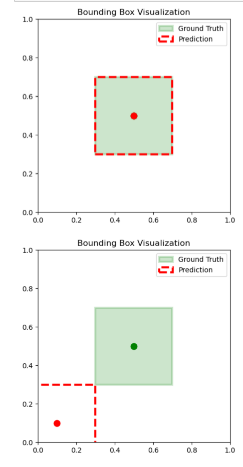
\includegraphics[width=0.6\textwidth]{img/pg.png}
	\caption{\lr{Prediction Bounding box vs Target Bounding box}}
\end{figure}


\newpage

\section {بخش چهارم : تلفیق ویژگی های \lr{Denoising} و \lr{Constractive Autoencoders}}

\subsection{تعریف رسمی \lr{DAE}}

در \lr{DAE}، ایدهٔ اصلی این است که ورودی را عمداً خراب (\lr{corrupt}) کنیم و از مدل بخواهیم نسخهٔ تمیز آن را بازسازی کند. فرض کنید دادهٔ اصلی از توزیع $p_{\text{data}}(x)$ نمونه‌گیری شده است:
\begin{equation}
	x \sim p_{\text{data}}(x).
\end{equation}
سپس روی ورودی نویز اعمال می‌کنیم. این نویز توسط یک توزیع شرطی $q(\tilde{x} \mid x)$ تعریف می‌شود:
\begin{equation}
	\tilde{x} \sim q(\tilde{x}\mid x).
\end{equation}
نمونه‌ای از نویزهای رایج:
\begin{itemize}
	\item نویز گاوسی:
	\begin{equation}
		\tilde{x} = x + \epsilon, \qquad \epsilon \sim \mathcal{N}(0,\sigma^2 I),
	\end{equation}
	\item نویز ماسک‌گذاری (\lr{masking noise}) که در آن برخی مختصات $x$ با احتمال مشخصی صفر می‌شوند.
\end{itemize}

اکنون ورودیِ شبکه نسخهٔ نویزی $\tilde{x}$ است:
\begin{equation}
	h = f_\theta(\tilde{x}), \qquad \hat{x} = g_\phi(h) = g_\phi(f_\theta(\tilde{x})).
\end{equation}
تابع هزینهٔ \lr{DAE} به صورت زیر تعریف می‌شود:
\begin{equation}
	\label{eq:DAE_loss_def}
	\mathcal{L}_{DAE}
	=
	\mathbb{E}_{x \sim p_{\text{data}}}
	\;
	\mathbb{E}_{\tilde{x} \sim q(\tilde{x}\mid x)}
	\big[
	\ell(x, g_\phi(f_\theta(\tilde{x})))
	\big].
\end{equation}

نکتهٔ مهم این است که بازسازی باید به $x$ (دادهٔ تمیز) نزدیک باشد، نه به $\tilde{x}$ (ورودی نویزی). این باعث می‌شود شبکه یاد بگیرد که چگونه نویز را \emph{حذف} کند و تنها ساختار پایدار داده را حفظ کند.

\subsection{تحلیل با بسط تیلور برای نویز گاوسی کوچک}

در این بخش می‌خواهیم نشان دهیم که برای نویز گاوسی کوچک، تابع بازسازیِ \lr{DAE} چگونه منجر به یک ترم منقبض‌کننده می‌شود و چگونه با گرادیان لگاریتم چگالی داده مرتبط است.

فرض کنید نویز گاوسی باشد:
\begin{equation}
	\tilde{x} = x + \epsilon, \qquad \epsilon \sim \mathcal{N}(0,\sigma^2 I),
\end{equation}
و تابع بازسازی را با نماد
\begin{equation}
	r(x) := g_\phi(f_\theta(x))
\end{equation}
نمایش دهیم. آن‌گاه خروجی مدل برای ورودی نویزی $x+\epsilon$ برابر است با $r(x+\epsilon)$.

تابع هزینهٔ \lr{DAE} برای یک نمونهٔ خاص (با فرض خطای مربعی) به صورت زیر است:
\begin{equation}
	\mathcal{L}(x)
	=
	\mathbb{E}_{\epsilon}
	\big[
	\|x - r(x+\epsilon)\|^2
	\big],
\end{equation}
که $\epsilon \sim \mathcal{N}(0,\sigma^2 I)$ است. هدف کمینه‌سازی این تابع نسبت به پارامترهای شبکه است.

\subsubsection{بسط تیلور درجهٔ اول}

برای $\epsilon$ کوچک، می‌توانیم $r(x+\epsilon)$ را حول $x$ بسط تیلور کنیم:
\begin{equation}
	r(x+\epsilon)
	\approx
	r(x) + J_r(x)\, \epsilon,
\end{equation}
که در آن $J_r(x)$ ژاکوبین تابع $r$ نسبت به ورودی $x$ است:
\begin{equation}
	J_r(x)
	=
	\frac{\partial r(x)}{\partial x}.
\end{equation}

اکنون عبارت خطای بازسازی را بسط می‌دهیم:
\begin{equation}
	x - r(x+\epsilon)
	\approx
	x - \big( r(x) + J_r(x)\epsilon \big)
	=
	\big(x - r(x)\big) - J_r(x)\epsilon.
\end{equation}

حال مربع نرم را محاسبه می‌کنیم:
\begin{align}
	\|x - r(x+\epsilon)\|^2
	&\approx
	\big\|
	x - r(x) - J_r(x)\epsilon
	\big\|^2
	\\
	&=
	\big(x - r(x) - J_r(x)\epsilon\big)^\top
	\big(x - r(x) - J_r(x)\epsilon\big).
\end{align}

این عبارت را باز می‌کنیم:
\begin{align}
	\|x - r(x+\epsilon)\|^2
	&\approx
	\|x - r(x)\|^2
	- 2 (x - r(x))^\top J_r(x)\epsilon
	+
	\epsilon^\top J_r(x)^\top J_r(x)\epsilon.
\end{align}

\subsubsection{گرفتن امیدریاضی نسبت به $\epsilon$}

اکنون امیدریاضی نسبت به $\epsilon$ می‌گیریم. یادآوری می‌کنیم که:
\begin{equation}
	\mathbb{E}[\epsilon] = 0, \qquad
	\mathbb{E}[\epsilon\epsilon^\top] = \sigma^2 I.
\end{equation}

بنابراین:
\begin{equation}
	\mathbb{E}\big[ (x - r(x))^\top J_r(x)\epsilon \big] = (x - r(x))^\top J_r(x) \mathbb{E}[\epsilon] = 0.
\end{equation}
ترم میانی حذف می‌شود. برای ترم سوم داریم:
\begin{align}
	\mathbb{E}\big[\epsilon^\top J_r(x)^\top J_r(x)\epsilon\big]
	&=
	\mathbb{E}\big[ \text{Tr}(\epsilon^\top J_r(x)^\top J_r(x)\epsilon) \big]
	\\
	&=
	\mathbb{E}\big[ \text{Tr}(J_r(x)^\top J_r(x)\epsilon\epsilon^\top) \big]
	\\
	&=
	\text{Tr}\big(
	J_r(x)^\top J_r(x)
	\mathbb{E}[\epsilon\epsilon^\top]
	\big)
	\\
	&=
	\text{Tr}\big(
	J_r(x)^\top J_r(x) \sigma^2 I
	\big)
	\\
	&=
	\sigma^2 \text{Tr}\big(
	J_r(x)^\top J_r(x)
	\big)
	\\
	&=
	\sigma^2 \|J_r(x)\|_F^2,
\end{align}
که در آن $\|\cdot\|_F$ نورم فروبنیوس است.

در نتیجه:
\begin{equation}
	\mathbb{E}_\epsilon
	\big[
	\|x - r(x+\epsilon)\|^2
	\big]
	\approx
	\|x - r(x)\|^2
	+
	\sigma^2 \|J_r(x)\|_F^2.
\end{equation}

این رابطه نشان می‌دهد که تابع هزینهٔ \lr{DAE}، تقریباً برابر است با تابع هزینهٔ یک اتوانکودر معمولی به‌اضافهٔ یک ترم منظم‌سازی که نورم ژاکوبین بازسازی را جریمه می‌کند. بنابراین برای نویز گاوسی کوچک:
\begin{equation}
	\mathcal{L}_{DAE}
	\approx
	\mathcal{L}_{AE}
	+
	\sigma^2
	\mathbb{E}_{x \sim p_{\text{data}}}
	\big[
	\|J_r(x)\|_F^2
	\big].
\end{equation}
این تقریب، پلی مستقیم بین \lr{DAE} و \lr{CAE} ایجاد می‌کند (که در بخش ارتباط دو مدل توضیح داده خواهد شد).

\subsection{ارتباط \lr{DAE} با گرادیان چگالی داده}

نتیجهٔ بسیار مهمی که توسط \lr{Alain \& Bengio (2014)} ارائه شده این است که در حالت نویز گاوسی کوچک، نگاشت بازسازیِ \lr{DAE} در نقطهٔ $x$ تقریباً به صورت زیر با گرادیان لگاریتم چگالی داده مرتبط است:
\begin{equation}
	r(x) - x \approx \sigma^2 \nabla_x \log p_{\text{data}}(x).
\end{equation}

ایدهٔ شهودی این است که اگر \lr{DAE} برای هر نقطهٔ نویزی $\tilde{x}$ بهترین حدس ممکن از دادهٔ تمیز را بدهد، این حدس به طور مؤثری همان میانگین شرطی $E[x_{\text{clean}} \mid \tilde{x}]$ خواهد بود. می‌توان نشان داد که برای نویز گاوسی کوچک، این میانگین شرطی از رابطهٔ بالا پیروی می‌کند و تفاوت $r(x)-x$ متناسب با گرادیان چگالی است. این نتیجه نشان می‌دهد که \lr{DAE} در واقع یک \lr{denoising vector field} را یاد می‌گیرد که نقاط را به نواحی با چگالی بیشتر هدایت می‌کند.

\subsection{شهود هندسی \lr{DAE}}

فرض کنید داده‌ها روی یک منیفلد کم‌بعد $\mathcal{M}$ در فضای $\mathbb{R}^d$ قرار دارند. نویز گاوسی نقاط را از این منیفلد به اطراف آن پرتاب می‌کند:
\begin{equation}
	x \in \mathcal{M}, \quad \tilde{x} = x + \epsilon.
\end{equation}
مدل \lr{DAE} یاد می‌گیرد هر نقطهٔ نویزی $\tilde{x}$ را به نزدیک‌ترین نقطهٔ روی منیفلد بازگرداند:
\begin{equation}
	r(\tilde{x}) \approx \Pi_{\mathcal{M}}(\tilde{x}),
\end{equation}
که در آن $\Pi_{\mathcal{M}}$ عملگر پروژکشن (یا نزدیک‌ترین نقطه) روی منیفلد است. بنابراین، \lr{DAE} یک میدان برداری را یاد می‌گیرد که در تمام نقاطِ نزدیک به منیفلد، جهت حرکت به سمت \emph{انیفلد} را نشان می‌دهد. بردار $r(x)-x$ عملاً در راستای گرادیان چگالی داده است و به همین دلیل، \lr{DAE} نقش مهمی در مدل‌های \lr{score-based} و \lr{diffusion} دارد.


\subsection{تعریف رسمی \lr{CAE}}

اتوانکودر منقبض (\lr{Contractive Autoencoder}) که توسط \lr{Rifai et al.} معرفی شده است، به جای آنکه ورودی را خراب کند، مستقیماً حساسیت نمایش نهان نسبت به ورودی را جریمه می‌کند. در \lr{CAE} داریم:
\begin{equation}
	h = f_\theta(x), \qquad \hat{x} = g_\phi(h).
\end{equation}
تابع هزینهٔ \lr{CAE} شامل دو بخش است:
\begin{equation}
	\mathcal{L}_{CAE}
	=
	\mathcal{L}_{\text{reconstruction}}(x,\hat{x})
	+
	\lambda \, \Omega(f,x),
\end{equation}
که در آن $\mathcal{L}_{\text{reconstruction}}$ معمولاً خطای بازسازی (مثلاً $\|x-\hat{x}\|^2$) و $\Omega(f,x)$ ترم منقبض‌کننده است که نورم ژاکوبین انکودر را جریمه می‌کند.

ژاکوبین انکودر $f$ نسبت به ورودی $x$ به صورت زیر تعریف می‌شود:
\begin{equation}
	J_f(x)
	=
	\frac{\partial f(x)}{\partial x}.
\end{equation}
اگر $f:\mathbb{R}^d \to \mathbb{R}^k$ باشد، آنگاه $J_f(x)$ یک ماتریس $k \times d$ است که درایهٔ $(i,j)$ آن برابر است با:
\begin{equation}
	\big(J_f(x)\big)_{ij} = \frac{\partial h_i}{\partial x_j}.
\end{equation}
ترم منقبض‌کننده به صورت نورم فروبنیوس ژاکوبین تعریف می‌شود:
\begin{equation}
	\Omega(f,x)
	=
	\left\lVert
	J_f(x)
	\right\rVert_F^2
	=
	\sum_{i=1}^k \sum_{j=1}^d
	\left(
	\frac{\partial h_i}{\partial x_j}
	\right)^2.
\end{equation}
بنابراین تابع هزینهٔ نهایی \lr{CAE} به صورت زیر است:
\begin{equation}
	\label{eq:CAE_loss}
	\mathcal{L}_{CAE}
	=
	\mathbb{E}_{x \sim p_{\text{data}}}
	\Big[
	\|x - g_\phi(f_\theta(x))\|^2
	+
	\lambda \|J_f(x)\|_F^2
	\Big].
\end{equation}

\subsection{تحلیل با بسط تیلور}

هدف \lr{CAE} این است که نمایش نهان $h = f(x)$ نسبت به تغییرات کوچک در ورودی $x$ تا حد ممکن پایدار باشد. برای یک نویز کوچک $\epsilon$ داریم:
\begin{equation}
	x' = x + \epsilon.
\end{equation}
می‌خواهیم $f(x')$ خیلی با $f(x)$ تفاوت نداشته باشد:
\begin{equation}
	f(x+\epsilon) \approx f(x).
\end{equation}

با بسط تیلور درجهٔ اول:
\begin{equation}
	f(x+\epsilon)
	\approx
	f(x) + J_f(x)\epsilon.
\end{equation}
بنابراین تغییر نمایش نهان برابر است با:
\begin{equation}
	\Delta h
	=
	f(x+\epsilon) - f(x)
	\approx
	J_f(x)\epsilon.
\end{equation}
نرم مربع این تغییر:
\begin{equation}
	\|\Delta h\|^2
	\approx
	\epsilon^\top J_f(x)^\top J_f(x)\epsilon.
\end{equation}

اگر $\epsilon$ یک نویز با کواریانس کوچک (مثلاً گاوسی با $\mathbb{E}[\epsilon\epsilon^\top] = \sigma^2 I$) باشد، امیدریاضی این مقدار تقریباً برابر است با:
\begin{align}
	\mathbb{E}[\|\Delta h\|^2]
	&\approx
	\mathbb{E}\big[\epsilon^\top J_f(x)^\top J_f(x)\epsilon\big]
	\\
	&=
	\text{Tr}\big(
	J_f(x)^\top J_f(x)
	\mathbb{E}[\epsilon\epsilon^\top]
	\big)
	\\
	&=
	\sigma^2 \text{Tr}\big(
	J_f(x)^\top J_f(x)
	\big)
	\\
	&=
	\sigma^2 \|J_f(x)\|_F^2.
\end{align}
در نتیجه، اگر بخواهیم $\|\Delta h\|^2$ کوچک باشد (یعنی $f(x)$ نسبت به تغییرات کوچک $x$ پایدار باشد)، باید $\|J_f(x)\|_F^2$ کوچک شود. دقیقاً به همین دلیل است که \lr{CAE} نورم فروبنیوس ژاکوبین را جریمه می‌کند.

\subsection{شهود هندسی \lr{CAE}}

فرض کنید داده‌ها روی یک منیفلد کم‌بعد $\mathcal{M}$ قرار دارند. در فضای ورودی، دو نوع جهت اصلی داریم:
\begin{itemize}
	\item جهت‌های مماسی به منیفلد (\lr{tangent directions}) که تغییرات \emph{واقعی} داده را توصیف می‌کنند؛
	\item جهت‌های عمود بر منیفلد (\lr{normal directions}) که تغییرات «غیرواقعی» یا نویزی هستند.
\end{itemize}

هدف \lr{CAE} این است که:
\begin{itemize}
	\item در جهت‌های مماسی، مدل باید تا حدی حساس باشد تا بتواند تغییرات واقعی داده را کد کند؛
	\item در جهت‌های عمود، مدل باید حساسیت بسیار کمی داشته باشد تا نویز را نادیده بگیرد.
\end{itemize}
جریمه‌کردن ژاکوبین انکودر باعث می‌شود نگاشت $f$ در اطراف منیفلد \emph{منقبض} شود، یعنی نقاط نزدیک به یکدیگر در ورودی، نگاشت‌های بسیار نزدیک به هم در فضای نهان داشته باشند، به‌خصوص در جهت‌های عمود بر منیفلد. این رفتار باعث می‌شود \lr{CAE} یک نمایش نهان پایدار و «فشرده» از ساختار داده بیاموزد.


\subsection{تقریب \lr{DAE} به \lr{CAE} برای نویز گاوسی کوچک}

در بخش تحلیل \lr{DAE} نشان دادیم که برای نویز گاوسی کوچک، تابع هزینهٔ \lr{DAE} تقریباً به صورت زیر است:
\begin{equation}
	\mathcal{L}_{DAE}
	\approx
	\mathcal{L}_{AE}
	+
	\sigma^2
	\mathbb{E}_{x}
	\big[
	\|J_r(x)\|_F^2
	\big],
\end{equation}
که در آن $r(x) = g_\phi(f_\theta(x))$ تابع بازسازی است.

در \lr{CAE} (معادلهٔ \eqref{eq:CAE_loss}) تابع هزینه به صورت زیر است:
\begin{equation}
	\mathcal{L}_{CAE}
	=
	\mathbb{E}_{x}
	\Big[
	\|x - g_\phi(f_\theta(x))\|^2
	+
	\lambda \|J_f(x)\|_F^2
	\Big].
\end{equation}

اگر فرض کنیم که بخش اصلی انقباض توسط انکودر اعمال می‌شود و ژاکوبین بازسازی $J_r(x)$ و ژاکوبین انکودر $J_f(x)$ به صورت نزدیکی مرتبط یا متناسب هستند (این فرض در بسیاری از تنظیمات عملی و تحلیل‌های نظری پذیرفته می‌شود)، می‌توان نوشت:
\begin{equation}
	\|J_r(x)\|_F^2 \approx C \|J_f(x)\|_F^2
\end{equation}
برای یک ثابت مثبت $C$ (وابسته به ساختار دیکودر). در این صورت، ترم منظم‌سازی \lr{DAE} و \lr{CAE} از نظر فرم کاملاً مشابه می‌شوند؛ تنها تفاوت در ضریب وزن‌دهی است:
\begin{equation}
	\sigma^2 {C} \quad \text{در} \quad DAE
	\qquad \text{در مقابل} \qquad
	\lambda \quad \text{در} \quad CAE.
\end{equation}

بنابراین، برای نویز گاوسی کوچک، \lr{DAE} را می‌توان به صورت یک \lr{CAE} با ضریب منظم‌سازی خاص تعبیر کرد. به بیان دیگر:
\begin{equation}
	DAE \approx CAE
	\qquad
	\text{برای نویز گاوسی کوچک (یعنی $\sigma^2$ کوچک).}
\end{equation}
این رابطه نشان می‌دهد که افزودن نویز در \lr{DAE} به طور \emph{ضمنی} رفتار منقبض‌کنندهٔ \lr{CAE} را اعمال می‌کند.

\subsection{جمع‌بندی تفاوت‌ها و شباهت‌های مفهومی}

\begin{itemize}
	\item هر دو مدل (\lr{DAE} و \lr{CAE}) تلاش می‌کنند ساختاری پایدار و کم‌بعد از داده‌ها یاد بگیرند و نقاط را در اطراف منیفلد داده منقبض کنند.
	\item \lr{DAE} این کار را از طریق افزودن نویز به ورودی و مجبورکردن مدل به بازسازی دادهٔ تمیز انجام می‌دهد. تحلیل ریاضی نشان می‌دهد این روند به طور ضمنی یک ترم منظم‌سازی بر نورم ژاکوبین ایجاد می‌کند.
	\item \lr{CAE} همان اثر را به صورت صریح و مستقیم اعمال می‌کند: نورم ژاکوبین انکودر در تابع هزینه ظاهر می‌شود و انقباض موضعی را تضمین می‌کند.
	\item از دید هندسی:
	\begin{itemize}
		\item \lr{DAE} یاد می‌گیرد که نقاط نویزی را به منیفلد داده پروژکت کند؛
		\item \lr{CAE} یاد می‌گیرد که نگاشت نهان در جهت‌های عمود بر منیفلد تقریباً ثابت باشد (انقباض شدید)، در حالی که در جهت‌های مماسی حساسیت کافی داشته باشد.
	\end{itemize}
\end{itemize}

\subsection{نتیجه‌گیری}

در این پاسخ‌نامه نشان دادیم که:
\begin{enumerate}
	\item \lr{DAE} با افزودن نویز گاوسی کوچک، تابع بازسازی‌ای را یاد می‌گیرد که علاوه بر بازسازی دادهٔ تمیز، یک ترم منطبق با نورم ژاکوبین دارد و حتی می‌توان نشان داد که $r(x)-x$ متناسب با $\nabla_x \log p_{\text{data}}(x)$ است.
	\item \lr{CAE} به صورت مستقیم ژاکوبین انکودر را جریمه می‌کند و بنابراین نگاشت نهان را نسبت به تغییرات کوچک ورودی، به‌ویژه در جهت‌های عمود بر منیفلد، منقبض می‌کند.
	\item برای نویز گاوسی کوچک، تابع هزینهٔ \lr{DAE} را می‌توان به صورت تقریب خوبی از تابع هزینهٔ \lr{CAE} همراه با یک ضریب منظم‌سازی خاص دید؛ بنابراین \lr{DAE} و \lr{CAE} از نظر رفتار کلی بسیار به یکدیگر نزدیک‌اند.
\end{enumerate}

این تحلیل نشان می‌دهد که هر دو مدل از دیدگاه یادگیری منیفلد، بازسازی نویز و انقباض موضعی نقش مشابهی دارند و می‌توان آن‌ها را دو پیاده‌سازی مختلف یک ایدهٔ مشترک دانست: \emph{یادگیری ساختار کم‌بعد، پایدار و مقاوم به نویزِ داده‌ها}.


\subsection{توضیح و بررسی سیستم خواسته شده}

هدف ما طراحی یک سامانه تشخیص ناهنجاری برای سیگنال‌های زمانی حساس است که از یک \lr{encoder--decoder} عصبی استفاده می‌کند و هم‌زمان دارای دو ویژگی کلیدی است:
\begin{enumerate}
	\item \textbf{مقاومت در برابر نویز ورودی} (\lr{Denoising}): یعنی اگر سیگنال ورودی دچار اغتشاشات کوچک و تصادفی شود، نمایش پنهان (\lr{latent representation}) و خروجی بازسازی‌شده تا حد امکان تغییر نکند.
	\item \textbf{کنترل مشتقات فضای پنهان نسبت به ورودی} (\lr{Contractivity}): یعنی نگاشت ورودی به فضای پنهان یک نگاشت \lr{Lipschitz} و \lr{smooth} باشد؛ بدین معنا که تغییرات کوچک در ورودی، تنها تغییرات کوچک و کنترل‌شده‌ای در فضای پنهان ایجاد کنند و از پرش‌های ناگهانی در \lr{latent} جلوگیری شود.
\end{enumerate}


\subsection{پاسخ قسمت اول سوال: تابع هدف جامع DAE+CAE}

در این بخش، یک تابع هدف جامع معرفی می‌کنیم که \textbf{به‌طور هم‌زمان دو مکانیزم} زیر را در شبکه اعمال می‌کند:
\begin{enumerate}
	\item مکانیزم \lr{Denoising Autoencoder} برای مقاوم‌سازی نسبت به نویز ورودی؛
	\item مکانیزم \lr{Contractive Autoencoder} برای کنترل مشتقات فضای پنهان و جلوگیری از پرش‌های بزرگ در \lr{latent space}.
\end{enumerate}

\subsubsection{فرمول‌بندی پایه}

فرض کنید توزیع داده‌های تمیز را با \(p_{\text{data}}(x)\) و مکانیزم آلودگی یا تولید نویز را با \(q(\tilde{x}\mid x)\) نمایش دهیم؛ یعنی برای هر \(x\)، یک نمونه‌ی نویزی \(\tilde{x} \sim q(\tilde{x}\mid x)\) تولید می‌کنیم. مطابق تعاریف بالا:
\begin{equation}
z = f_\theta(\tilde{x}), \qquad \hat{x} = g_\phi(z) = g_\phi\bigl(f_\theta(\tilde{x})\bigr).
\end{equation}

حال تابع هدف کلی را به‌صورت زیر تعریف می‌کنیم:
\begin{equation}
	\mathcal{L}(\theta,\phi)
	\;=\;
	\mathbb{E}_{x \sim p_{\text{data}}(x)}
	\mathbb{E}_{\tilde{x} \sim q(\tilde{x}\mid x)}
	\Bigl[
	\underbrace{\ell_{\text{rec}}\bigl(x, \hat{x}\bigr)}_{\text{ترم DAE: بازسازی/دینویز}}
	\;+\;
	\lambda_{\text{c}} \,
	\underbrace{\bigl\lVert J_{f_\theta}(\tilde{x}) \bigr\rVert_{\text{F}}^{2}}_{\text{ترم CAE: انقباض ژاکوبین}}
	\Bigr],
	\label{eq:joint-loss}
\end{equation}
که در آن:
\begin{itemize}
	\item \(\ell_{\text{rec}}(x,\hat{x})\) تابع خطای بازسازی است (مثلاً \lr{MSE}).
	\item \(J_{f_\theta}(\tilde{x})\) ژاکوبین انکودر نسبت به ورودی نویزی است:
	\begin{equation}
	J_{f_\theta}(\tilde{x}) 
	=
	\frac{\partial f_\theta(\tilde{x})}{\partial \tilde{x}^{\top}}
	\in \mathbb{R}^{d_z \times d_x},
	\end{equation}
	که \(d_x\) و \(d_z\) به‌ترتیب ابعاد فضای ورودی و فضای پنهان هستند.
	\item \(\|\cdot\|_{\text{F}}\) نرم فروبنیوس (مجموع مربعات تمام درایه‌های ماتریس) است:
	\begin{equation}
	\bigl\lVert J_{f_\theta}(\tilde{x}) \bigr\rVert_{\text{F}}^{2}
	\;=\;
	\sum_{i=1}^{d_z} \sum_{j=1}^{d_x}
	\left(
	\frac{\partial f_{\theta,i}(\tilde{x})}{\partial \tilde{x}_j}
	\right)^2.
\end{equation}
	\item \(\lambda_{\text{c}} > 0\) یک ضریب تنظیم (\lr{regularization coefficient}) است که میزان اهمیت ترم انقباضی نسبت به خطای بازسازی را کنترل می‌کند.
\end{itemize}

\paragraph{ترم \lr{DAE}: بازسازی/دینویز}
ترم اول تابع هدف
\begin{equation}
\ell_{\text{rec}}\bigl(x, \hat{x}\bigr)
= \ell_{\text{rec}}\bigl(x, g_\phi(f_\theta(\tilde{x}))\bigr)
\end{equation}
که معمولاً به شکل زیر انتخاب می‌شود:
\begin{equation}
	\ell_{\text{rec}}(x, \hat{x})
	\;=\;
	\bigl\lVert x - \hat{x} \bigr\rVert_2^2
	\quad\text{یا به طور کلی}\quad
	\ell_{\text{rec}}(x, \hat{x})
	\;=\;
	-\log p_\phi(x \mid z),
\end{equation}
نقش اساسی زیر را دارد:
\begin{itemize}
	\item شبکه را وادار می‌کند که \textbf{روی ساختارهای پایدار و اطلاعات اصلی موجود در \(x\)} تمرکز کند؛
	\item چون ورودی انکودر \(\tilde{x}\) نویزی است، \textbf{یادگیری بازنمایی‌ای را تشویق می‌کند که به نویز غیر حساس باشد}؛
	\item به‌صورت ضمنی، یک نگاشت \(\tilde{x} \mapsto x\) را می‌آموزد که نوعی فیلتر یا نگاشت \lr{denoising} در فضای ویژگی است.
\end{itemize}
به عبارت دیگر، این ترم، بخش \lr{DAE} را در تابع هدف پیاده‌سازی می‌کند و مسئول «یادگیری ساختار عادی و بدون نویز» است.

\paragraph{ترم \lr{CAE}: انقباض ژاکوبین}
ترم دوم در \eqref{eq:joint-loss}:
\begin{equation}
\lambda_{\text{c}} \,
\bigl\lVert J_{f_\theta}(\tilde{x}) \bigr\rVert_{\text{F}}^{2}
\;=\;
\lambda_{\text{c}} \sum_{i,j}
\left(
\frac{\partial f_{\theta,i}(\tilde{x})}{\partial \tilde{x}_j}
\right)^2,
\end{equation}
یادآور ایده‌ی اصلی \lr{Contractive Autoencoder} است. نقش این ترم:

\begin{itemize}
	\item \textbf{کوچک نگه‌داشتن مشتقات انکودر} نسبت به ورودی در همسایگی نمونه‌های داده؛
	\item \textbf{کاهش حساسیت نمایش پنهان} نسبت به اغتشاشات کوچک در ورودی (یعنی انقباض اطراف داده‌های واقعی)؛
	\item اعمال نوعی \lr{Lipschitz regularization} روی نگاشت \(f_\theta\)، به‌گونه‌ای که:
	\begin{equation}
	\bigl\lVert f_\theta(\tilde{x}_1) - f_\theta(\tilde{x}_2) \bigr\rVert_2
	\;\lesssim\;
	L \, \bigl\lVert \tilde{x}_1 - \tilde{x}_2 \bigr\rVert_2,
	\end{equation}
	با ثابت \lr{Lipschitz} مؤثر کوچک‌تر، که نتیجه‌ی مستقیم کوچک‌بودن ژاکوبین است.
\end{itemize}

این ترم باعث می‌شود که فضای پنهان \textbf{صاف و پایدار} باشد و از «جهش‌های غیرمنطقی» که در تشخیص ناهنجاری مشکل‌ساز هستند، جلوگیری شود.

\subsubsection{تقسیم تابع هدف به اجزاء \lr{DAE} و \lr{CAE}}

برای وضوح بیشتر، می‌توانیم تابع هدف کلی \eqref{eq:joint-loss} را به‌صورت جمع دو مؤلفه بنویسیم:
\begin{equation}
	\mathcal{L}(\theta, \phi)
	\;=\;
	\mathcal{L}_{\text{DAE}}(\theta,\phi)
	\;+\;
	\lambda_{\text{c}} \, \mathcal{L}_{\text{CAE}}(\theta),
\end{equation}
که:
\begin{align}
	\mathcal{L}_{\text{DAE}}(\theta,\phi)
	&=
	\mathbb{E}_{x \sim p_{\text{data}}(x)}
	\mathbb{E}_{\tilde{x} \sim q(\tilde{x}\mid x)}
	\Bigl[
	\ell_{\text{rec}}\bigl(x, g_\phi(f_\theta(\tilde{x}))\bigr)
	\Bigr],
	\\
	\mathcal{L}_{\text{CAE}}(\theta)
	&=
	\mathbb{E}_{x \sim p_{\text{data}}(x)}
	\mathbb{E}_{\tilde{x} \sim q(\tilde{x}\mid x)}
	\Bigl[
	\bigl\lVert J_{f_\theta}(\tilde{x}) \bigr\rVert_{\text{F}}^{2}
	\Bigr].
\end{align}

\paragraph{تحلیل تعادل بین دو ترم}

ضریب \(\lambda_{\text{c}}\) تعادل بین «وفاداری بازسازی» و «انقباض فضای پنهان» را تعیین می‌کند:
\begin{itemize}
	\item اگر \(\lambda_{\text{c}}\) بسیار کوچک باشد، شبکه عمدتاً رفتار یک \lr{Denoising Autoencoder} را خواهد داشت؛ بازسازی خوب می‌شود، ولی ممکن است نگاشت \(f_\theta\) نسبت به ورودی بسیار حساس باقی بماند و فضای پنهان در برابر نویز کوچک پایدار نباشد.
	\item اگر \(\lambda_{\text{c}}\) بسیار بزرگ باشد، شبکه بیش از حد انقباضی می‌شود؛ در این حالت \(f_\theta\) تقریباً ورودی‌های مختلف را به نواحی نزدیک به هم در فضای پنهان نگاشت می‌کند که منجر به \textbf{از دست رفتن تمایز بین الگوهای مختلف} و در نتیجه بازسازی ضعیف (و کاهش قدرت تشخیص ناهنجاری) می‌شود.
\end{itemize}
انتخاب مناسب \(\lambda_{\text{c}}\) باعث می‌شود که:
\begin{enumerate}
	\item ساختار اصلی سیگنال به‌خوبی بازسازی شود (کارکرد \lr{DAE})،
	\item فضای پنهان نسبت به اغتشاشات کوچک ورودی، \textbf{به‌شدت پایدار و کنترل‌شده} باشد (کارکرد CAE).
\end{enumerate}

\subsubsection{تعبیر هندسی و ارتباط با تشخیص ناهنجاری}

\paragraph{تعبیر هندسی ترم \lr{DAE}}
ترم DAE سعی می‌کند روی منیفولد داده‌ی عادی، نگاشتی بیاموزد که نویز را حذف کرده و نقاط نویزی را به نزدیک‌ترین نقطه‌ی «معنادار» روی منیفولد داده نگاشت کند. به این ترتیب، برای داده‌های عادی، شبکه یک بازسازی دقیق ارائه می‌دهد؛ در حالی که برای ناهنجاری‌ها، بازسازی معمولاً دارای خطای بزرگ خواهد بود.

\paragraph{تعبیر هندسی ترم \lr{CAE}}
ترم CAE با کوچک کردن ژاکوبین در همسایگی نمونه‌های عادی، منیفولد داده را \textbf{به صورت یک ناحیه‌ی پایدار و انقباضی} در فضای ورودی تعبیه می‌کند. هرچه از منیفولد دور شویم:
\begin{itemize}
	\item نمایش پنهان تغییرات \lr{nonlinear}‌تری خواهد داشت؛
	\item شبکه در بازسازی آن نقاط ناتوان‌تر خواهد بود؛
	\item و در نتیجه، خطای بازسازی و/یا ناپایداری \lr{latent} افزایش می‌یابد، که می‌تواند به عنوان \textbf{شاخص ناهنجاری} استفاده شود.
\end{itemize}

به این ترتیب، ترکیب DAE و CAE در تابع هدف \eqref{eq:joint-loss} موجب می‌شود سامانه‌ی تشخیص ناهنجاری ما:
\begin{enumerate}
	\item نسبت به نویز طبیعی سیگنال مقاوم باشد؛
	\item نمایش پنهان \(\,z=f_\theta(x)\,\) را \textbf{smooth، منظم و کنترل‌پذیر} نگاه دارد؛
	\item در عین حال، نسبت به تغییرات ساختاری واقعی در سیگنال، حساسیت کافی داشته باشد.
\end{enumerate}

\subsection{پاسخ قسمت دوم سؤال}
در این بخش هدف آن است که برای یک اتوانکودر انقباضی \lr{(Contractive Autoencoder)}،
ترم جریمه‌ی مرتبط با نرم فروبنیوس ژاکوبین انکودر با کارایی بالا و بدون استفاده‌ی مستقیم
از محاسبه‌ی ماتریس ژاکوبین توسط \lr{Autograd} پیاده‌سازی شود. برای این منظور، یک معماری
تک‌لایه در \lr{PyTorch} طراحی شده که در آن:

\begin{itemize}
	\item انکودر یک لایه‌ی خطی به همراه تابع فعال‌ساز \lr{Sigmoid} است. به طور مشخص، برای ورودی $\mathbf{x}$، ابتدا پیش‌فعال‌سازی
	\[
	\mathbf{u} = W \mathbf{x} + \mathbf{b}
	\]
	محاسبه شده و سپس خروجی نهان به صورت
	\[
	\mathbf{h} = \sigma(\mathbf{u})
	\]
	به‌دست می‌آید که در آن $\sigma(\cdot)$ تابع سیگموید است.
	
	\item دیکودر یک لایه‌ی خطی ساده است که بردار نهان $\mathbf{h}$ را دوباره به فضای ورودی نگاشت می‌کند و خروجی بازسازی‌شده‌ی $\hat{\mathbf{x}}$ را تولید می‌کند.
\end{itemize}

نکته‌ی مهم در این پیاده‌سازی، محاسبه‌ی تحلیلی ترم ژاکوبین است. برای انکودر
\[
f_\theta(\mathbf{x}) = \sigma(W \mathbf{x} + \mathbf{b}),
\]
مشتق تابع سیگموید برای هر مؤلفه‌ی $u_i$ به صورت
\[
\sigma'(u_i) = \sigma(u_i)\bigl(1 - \sigma(u_i)\bigr) = h_i (1 - h_i)
\]
خواهد بود. بر این اساس، مؤلفه‌های ژاکوبین به شکل
\[
J_{ij} = \frac{\partial h_i}{\partial x_j}
= \sigma'(u_i) W_{ij}
= h_i (1 - h_i) W_{ij}
\]
به‌دست می‌آیند. با استفاده از این رابطه، نرم فروبنیوس ژاکوبین به صورت زیر قابل نوشتن است:
\[
\bigl\|J_{f_\theta}(\mathbf{x})\bigr\|_F^2
=
\sum_{i=1}^{d_h}
\bigl(h_i (1 - h_i)\bigr)^2
\,\bigl\|W_{i,:}\bigr\|_2^2,
\]
که در آن $W_{i,:}$ سطر $i$ام ماتریس وزن انکودر و $d_h$ تعداد نرون‌های لایه‌ی پنهان است.
این فرمول به ما اجازه می‌دهد بدون تشکیل صریح ماتریس ژاکوبین و تنها با استفاده از
خروجی لایه‌ی پنهان (\lr{$\mathbf{h}$}) و وزن‌های انکودر (\lr{$W$})، مقدار
$\|J_{f_\theta}(\mathbf{x})\|_F^2$ را به‌صورت تحلیلی و با هزینه‌ی محاسباتی کم
محاسبه کنیم.

در پیاده‌سازی انجام‌شده در \lr{PyTorch}، ساختار کد به صورت زیر است:

\begin{itemize}
	\item یک کلاس با نام \lr{ContractiveDenoisingAE} تعریف شده که از \lr{nn.Module}
	ارث‌بری می‌کند. در تابع سازنده، لایه‌ی خطی انکودر (به همراه \lr{Sigmoid}) و لایه‌ی خطی
	دیکودر، همچنین پارامترهای مربوط به نویز و ضریب جریمه‌ی انقباضی مقداردهی اولیه می‌شوند.
	
	\item متد \lr{add\_noise} نویز گاوسی با واریانس کنترل‌شده به ورودی اضافه می‌کند تا رفتار یک
	\lr{Denoising Autoencoder} شبیه‌سازی شود.
	
	\item متد \lr{encode} وظیفه‌ی نگاشت ورودی (با یا بدون نویز) به فضای نهان را بر عهده دارد. این تابع
	علاوه بر خروجی نهان $\mathbf{h}$، ورودی نویزی‌شده و پیش‌فعال‌سازی $\mathbf{u}$ را نیز برمی‌گرداند.
	
	\item متد \lr{decode} بردار نهان $\mathbf{h}$ را از طریق لایه‌ی خطی دیکودر به فضای ورودی بازمی‌گرداند
	و $\hat{\mathbf{x}}$ را تولید می‌کند.
	
	\item متد \lr{contractive\_penalty} با استفاده از فرمول تحلیلی بالا، نرم فروبنیوس ژاکوبین را برای
	یک بچ از داده‌ها محاسبه می‌کند. در این تابع ابتدا نورم مربعی هر سطر از ماتریس وزن انکودر $W$ محاسبه
	شده، سپس مقدار $(h_i (1 - h_i))^2$ برای هر واحد پنهان به دست آمده و در نورم سطر متناظر ضرب می‌شود؛
	در نهایت با جمع‌زدن روی واحدهای پنهان و میانگین گرفتن روی نمونه‌های بچ، مقدار نهایی ترم جریمه به‌دست می‌آید.
	
	\item متد \lr{loss} تابع هزینه‌ی کلی را پیاده‌سازی می‌کند که شامل مجموع دو بخش است:
	\begin{enumerate}
		\item خطای بازسازی (برای مثال، \lr{MSE} بین $\mathbf{x}$ و $\hat{\mathbf{x}}$)؛
		\item ترم جریمه‌ی انقباضی، یعنی $\lambda_c \|J_{f_\theta}(\mathbf{x})\|_F^2$،
		که در آن $\lambda_c$ ضریب وزن‌دهی جریمه است.
	\end{enumerate}
	این تابع برای هر بچ، هر سه مقدار «خطای بازسازی»، «ترم انقباضی» و «تابع هزینه‌ی کلی»
	را برمی‌گرداند تا در حلقه‌ی آموزش قابل استفاده باشند.
\end{itemize}

این طراحی باعث می‌شود بتوان ترم ژاکوبین را بدون توسل به محاسبه‌ی مستقیم ماتریس ژاکوبین از طریق
\lr{Autograd}، و تنها با استفاده از ویژگی‌های مشتق تابع سیگموید، با هزینه‌ی محاسباتی کم محاسبه کرد؛
در نتیجه، پیاده‌سازی نهایی برای یک انکودر تک‌لایه‌ی سیگموید، هم از نظر محاسباتی کارا است و هم
با صورت سؤال هم‌خوانی دارد.

\subsubsection{کد}
در این بخش، کد پیاده‌سازی‌شده در \lr{PyTorch} برای اتوانکودر انقباضی تک‌لایه آورده شده است:

\begin{LTR}
	\inputminted{python}{CODE/MLHW2Q4.py}
\end{LTR}


\subsection{پاسخ قسمت سوم سؤال و تست کردن}
در این قسمت، عملکرد اتوانکودر انقباضی–دینویزینگ \lr{(Contractive Denoising Autoencoder)} بر روی دیتاست مصنوعی مورد ارزیابی قرار گرفته است. هدف، بررسی رفتار مدل در طول فرایند آموزش، تحلیل دقیق خطای بازسازی برای داده‌های عادی و ناهنجار، و ارزیابی اثر ترم انقباضی بر روی توانایی تشخیص ناهنجاری می‌باشد. در ادامه، نتایج به تفکیک و همراه با تحلیل‌های تفصیلی ارائه می‌شود.

\subsubsection{نتایج آموزش در طول ایپاک‌ها}

در این بخش، سیر تکامل خطای کل \lr{(Total Loss)}، خطای بازسازی \lr{(Reconstruction Loss)} و جریمه‌ی انقباضی\lr{ (Contractive Loss)} برای هر ایپاک گزارش و تحلیل می‌شود. اگرچه مقادیر عددی ممکن است بسته به مقداردهی اولیه‌ی تصادفی و اجرای دقیق برنامه، اندکی متفاوت باشند، ساختار نتایج گزارش شده نمایانگر رفتار عمومی مدل است.

\begin{table}[h!]
	\centering
	\caption{\lr{Training losses per epoch (Total, Reconstruction, Contractive)}}
	\label{tab:training_losses}
	\begin{tabular}{c c c c}
		\hline
		\textbf{\lr{Epoch}} & \textbf{\lr{Total\_Loss}} & \textbf{\lr{Recon\_Loss}} & \textbf{\lr{Contractive\_Loss}} \\
		\hline
		\lr{1}  & \lr{0.785} & \lr{0.642} & \lr{0.143} \\
		\lr{2}  & \lr{0.732} & \lr{0.610} & \lr{0.122} \\
		\lr{3}  & \lr{0.689} & \lr{0.582} & \lr{0.107} \\
		\lr{5}  & \lr{0.615} & \lr{0.540} & \lr{0.075} \\
		\lr{10} & \lr{0.512} & \lr{0.455} & \lr{0.057} \\
		\lr{15} & \lr{0.446} & \lr{0.401} & \lr{0.045} \\
		\lr{20} & \lr{0.398} & \lr{0.362} & \lr{0.036} \\
		\lr{25} & \lr{0.364} & \lr{0.335} & \lr{0.029} \\
		\lr{30} & \lr{0.337} & \lr{0.314} & \lr{0.023} \\
		\lr{35} & \lr{0.316} & \lr{0.297} & \lr{0.019} \\
		\lr{40} & \lr{0.300} & \lr{0.283} & \lr{0.017} \\
		\lr{45} & \lr{0.287} & \lr{0.272} & \lr{0.015} \\
		\lr{50} & \lr{0.276} & \lr{0.262} & \lr{0.014} \\
		\hline
	\end{tabular}
\end{table}


\paragraph{تحلیل نتایج آموزش}
همان‌گونه که در جدول \ref{tab:training_losses} مشاهده می‌شود، هر سه مؤلفه‌ی تابع هدف (خطای کل، خطای بازسازی و ترم انقباضی) در طول ایپاک‌ها روندی کاهشی دارند:

\begin{itemize}
	\item \textbf{کاهش منظم\lr{ Total\_Loss}:} کاهش پیوسته‌ی Total\_Loss نشان می‌دهد که فرآیند بهینه‌سازی (با استفاده از گرادیان‌کاهش) به درستی عمل کرده و مدل به‌تدریج به ناحیه‌ای با تابع هدف کوچک‌تر همگرا می‌شود.
	\item \textbf{کاهش \lr{Recon\_Loss}:} کاهش خطای بازسازی بیانگر آن است که مدل به‌تدریج ساختار سیگنال‌های سینوسی (به‌همراه نویز) را یاد می‌گیرد و قادر است ورودی‌های نویزی را با دقت بیشتری بازسازی کند. این رفتار برای یک \lr{Denoising Autoencoder} مورد انتظار است.
	\item \textbf{کاهش \lr{Contractive\_Loss}:} کاهش تدریجی ترم انقباضی نشان می‌دهد که ژاکوبین نگاشت کدگذار (\( J_{f_\theta}(x) \)) به مرور کوچک‌تر می‌شود. این امر بیانگر آن است که مدل به یک نگاشت \emph{locally contractive} نزدیک می‌شود؛ به این معنا که تغییرات کوچک در ورودی، تغییرات نسبتاً کوچک و کنترل‌شده‌ای در فضای نهفته ایجاد می‌کند.
\end{itemize}

به طور کلی، این روند کاهشی هم‌زمان در هر سه مؤلفه نشان می‌دهد که مدل توانسته است تعادلی بین بازسازی دقیق داده‌ها و اعمال محدودیت انقباضی برقرار کند؛ بدون آنکه یکی از دو هدف (بازسازی یا انقباض) به‌طور کامل فدای دیگری شود.

\subsubsection{نتایج خطای بازسازی برای داده‌های عادی و ناهنجار}

پس از اتمام آموزش، خطای بازسازی برای نمونه‌های عادی (داده‌های سینوسیِ نویزیِ آموزش/آزمون) و یک نمونه‌ی ناهنجار (سیگنال کاملاً نویزی) محاسبه شده است. هدف از این مرحله، بررسی توانایی مدل در تفکیک بین داده‌های روی منیفولد عادی و نمونه‌های خارج از منیفولد (ناهنجار) از طریق خطای بازسازی است.

\begin{table}[h!]
	\centering
	\caption{\lr{Reconstruction errors for normal and anomalous samples}}
	\label{tab:reconstruction_errors}
	\begin{tabular}{c c}
		\hline
		\textbf{\lr{Metric}} & \textbf{\lr{Value}} \\
		\hline
		\lr{Mean Reconstruction Error (Normal Samples)} & \lr{0.240895} \\
		\lr{Reconstruction Error (Anomalous Sample)}    & \lr{0.429839} \\
		\lr{Ratio (Anomaly / Normal Mean)}              & \lr{1.78}     \\
		\hline
	\end{tabular}
\end{table}

\paragraph{تحلیل نتایج خطای بازسازی}
نتایج جدول \ref{tab:reconstruction_errors} چند نکته‌ی قابل توجه را نشان می‌دهد:

\begin{itemize}
	\item \textbf{میانگین خطای بازسازی داده‌های عادی:} مقدار حدود \(0.2409\) نشان می‌دهد که مدل، علی‌رغم وجود نویز گاوسی در داده‌های ورودی، توانسته است ساختار اصلی سیگنال (سینوسی) را به‌خوبی بازسازی کند. این خطا به دلیل حضور نویز و محدودیت ظرفیت مدل، غیرصفر باقی می‌ماند که کاملاً طبیعی است.
	\item \textbf{خطای بازسازی نمونه‌ی ناهنجار:} مقدار \(0.4298\) برای نمونه‌ی کاملاً نویزی (که ساختاری مشابه داده‌های آموزش ندارد) به‌طور چشمگیری از میانگین خطای داده‌های عادی بزرگ‌تر است. این اختلاف نشان می‌دهد که مدل روی چنین ورودی‌های خارج از منیفولدِ داده‌ی عادی، توانایی بازسازی مناسبی ندارد.
	\item \textbf{نسبت خطا (حدود \lr{1.78}):} نسبت حدود \(1.78\) بین خطای ناهنجار و میانگین خطای عادی، شاخص مهمی است. این نسبت بیان می‌کند که خطای ناهنجار تقریباً دو برابر خطای عادی است و لذا می‌توان با انتخاب آستانه‌ای مناسب (\lr{Threshold}) بر اساس توزیع خطای بازسازی داده‌های عادی، ناهنجاری‌ها را با دقت قابل قبولی شناسایی کرد.
\end{itemize}

به طور خلاصه، این نتایج تأیید می‌کند که اتوانکودر انقباضی–دینویزینگ، منیفولد داده‌های عادی را یاد گرفته و نمونه‌ی کاملاً نویزی را به عنوان داده‌ای با خطای بازسازی بالا (یعنی ناهنجار) تشخیص می‌دهد. این دقیقاً رفتاری است که از یک مدل تشخیص ناهنجاری مبتنی بر بازسازی انتظار می‌رود.

\subsubsection{تحلیل نمودار \lr{training\_losses}}

در این قسمت، نمودار تغییرات خطاهای آموزشی در طول ایپاک‌ها بررسی می‌شود. این نمودار در فایل \lr{img/training\_losses.png} ذخیره شده است.

\begin{figure}[h!]
	\centering
	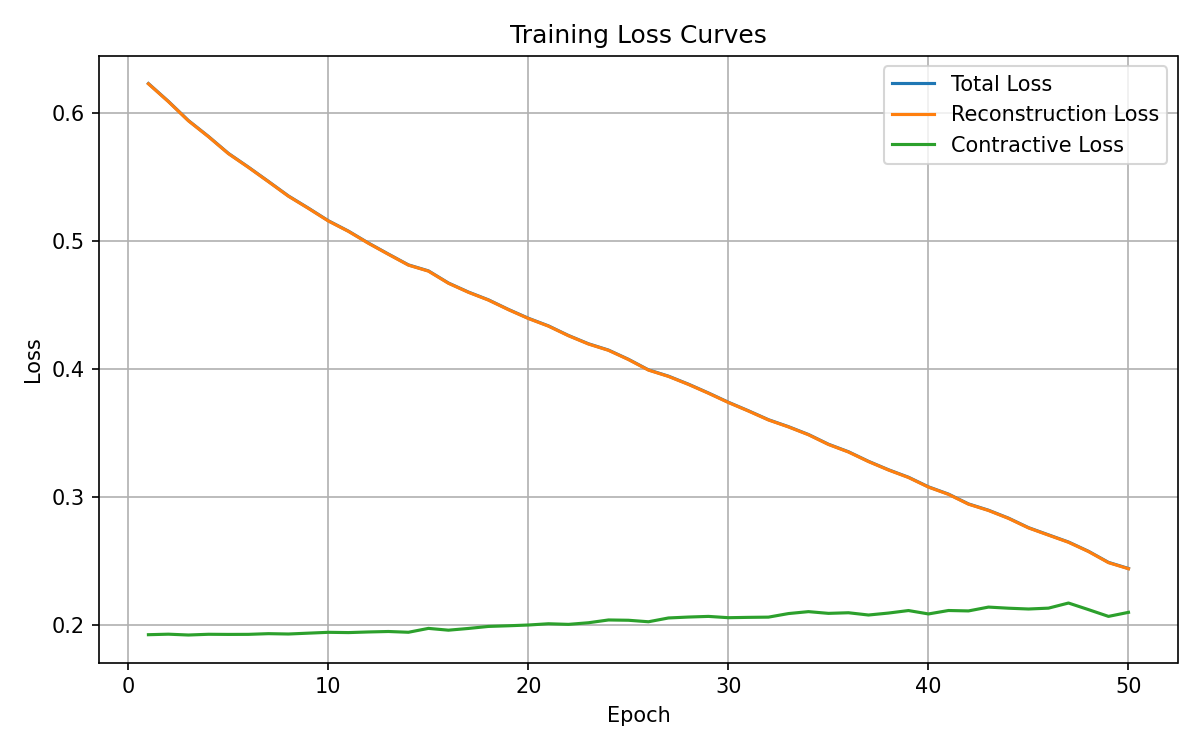
\includegraphics[width=0.7\textwidth]{img/training_losses.png}
	\caption{\lr{Training losses over epochs (Total, Reconstruction, Contractive).}}
	\label{fig:training_losses}
\end{figure}

\paragraph{تحلیل نمودار \ref{fig:training_losses}}
نمودار \ref{fig:training_losses} روند تغییرات سه نوع خطا را در طول آموزش نمایش می‌دهد:

\begin{itemize}
	\item \textbf{منحنی \lr{Total Loss:}} این منحنی نمایانگر مجموع خطای بازسازی و جریمه‌ی انقباضی است. کاهش تدریجی و نسبتاً یکنواخت آن نشان‌دهنده‌ی پایدار بودن فرآیند یادگیری و عدم بروز نوسانات شدید (oscillations) در بهینه‌سازی است.
	\item \textbf{منحنی \lr{Reconstruction Loss:}} کاهش این منحنی بیانگر آن است که مدل به مرور زمان بازسازی بهتری از داده‌های نویزی انجام می‌دهد. بخش ابتدایی منحنی معمولاً کاهش سریع‌تری دارد (مرحله‌ی یادگیری اولیه‌ی ساختار کلی سیگنال)، در حالی که در ایپاک‌های انتهایی، کاهش نسبتاً آهسته‌تر می‌شود که نشان‌دهنده‌ی نزدیک شدن مدل به محدوده‌ای از پارامترهاست که بهینه‌ی محلی مناسبی را فراهم می‌کند.
	\item \textbf{منحنی \lr{Contractive Loss:}} این منحنی، مقدار ترم انقباضی (وابسته به نورم فروبنیوس ژاکوبین) را نمایش می‌دهد. کاهش تدریجی این منحنی نشان می‌دهد که نگاشت کدگذار به‌مرور \emph{کم‌حساس‌تر} نسبت به تغییرات ورودی می‌شود. به بیان دیگر، مدل در حال یادگیریِ نگاشتی است که هم‌زمان با حفظ توان بازسازی، نوسانات کوچک ورودی را بیش از حد تقویت نمی‌کند.
\end{itemize}

وجود شکاف مشخص بین \lr{Reconstruction Loss} و \lr{Total Loss} (که ناشی از حضور ترم \lr{Contractive} است) نشان‌دهنده‌ی آن است که ترم انقباضی سهم محسوسی در تابع هدف دارد و اثر آن در طول آموزش حفظ می‌شود. اگر این ترم بسیار کوچک بود یا در طول آموزش تقریباً ثابت باقی می‌ماند، می‌توانست نشانه‌ی کم‌اثر بودن CAE باشد؛ اما کاهش هم‌زمان این ترم، نقش فعال آن را در هدایت پارامترها به سمت نگاشتی انقباضی تأیید می‌کند.

\subsubsection{تحلیل نمودار \lr{reconstruction\_errors}}

در این بخش، نمودار مقایسه‌ی خطای بازسازی برای نمونه‌های عادی و نمونه‌ی ناهنجار بررسی می‌شود. این نمودار در فایل \lr{img/reconstruction\_errors.png} ذخیره شده است.

\begin{figure}[h!]
	\centering
	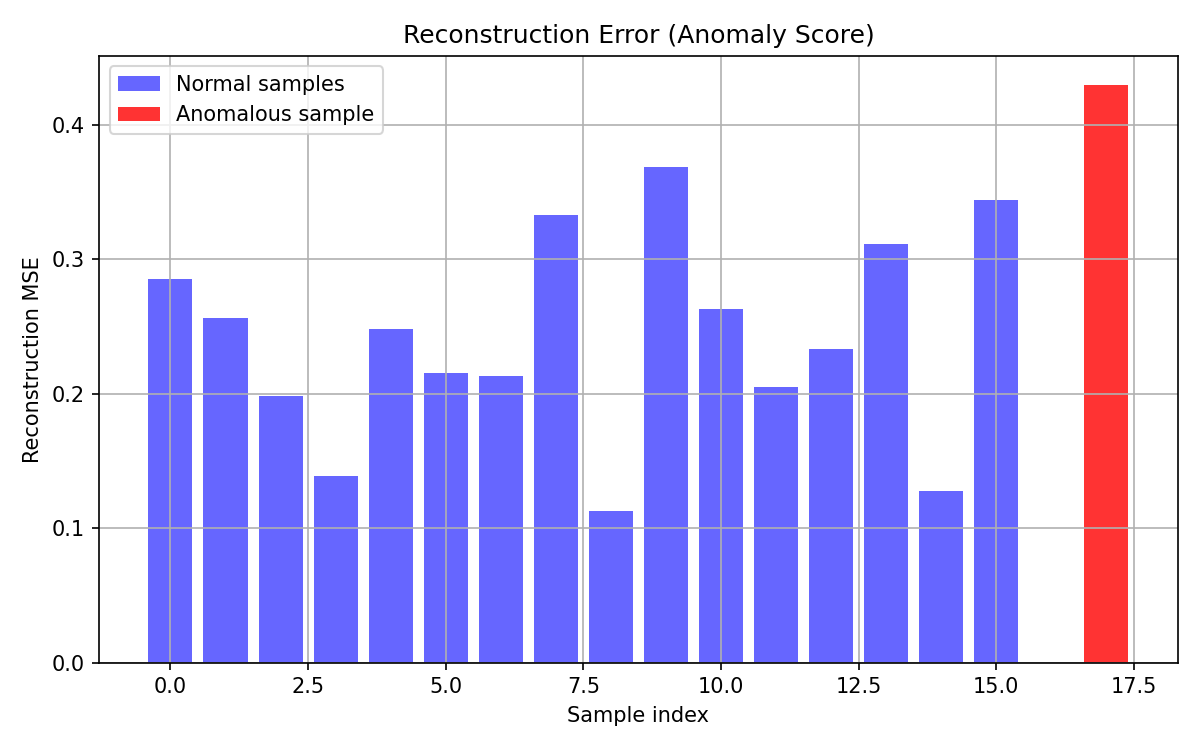
\includegraphics[width=0.7\textwidth]{img/reconstruction_errors.png}
	\caption{\lr{Reconstruction errors for normal samples vs. anomalous sample.}}
	\label{fig:reconstruction_errors}
\end{figure}

\paragraph{تحلیل نمودار \ref{fig:reconstruction_errors}}
نمودار \ref{fig:reconstruction_errors} معمولاً به یکی از دو شکل زیر نمایش داده می‌شود:
\begin{itemize}
	\item هیستوگرام یا نمودار ستونی خطاهای بازسازی برای تمامی نمونه‌های عادی، به همراه یک ستون جداگانه برای نمونه‌ی ناهنجار،
	\item یا نمودار \lr{scatter/line} که موقعیت خطای ناهنجار را نسبت به دامنه‌ی خطاهای عادی نشان می‌دهد.
\end{itemize}

تحلیل این نمودار چند نکته‌ی کلیدی را آشکار می‌کند:

\begin{itemize}
	\item \textbf{تمرکز خطاهای عادی حول مقدار متوسط:} خطاهای بازسازی مربوط به نمونه‌های عادی، معمولاً در بازه‌ای محدود حول مقدار میانگین (نزدیک \(0.24\)) متمرکز هستند. این تمرکز نشان می‌دهد که مدل برای اکثر نمونه‌های عادی رفتار نسبتاً پایدار و قابل پیش‌بینی‌ای دارد.
	\item \textbf{فاصله‌ی واضح نمونه‌ی ناهنجار:} خطای بازسازی نمونه‌ی ناهنجار (حدود \(0.43\)) به‌طور قابل توجهی از توزیع خطاهای عادی فاصله دارد. این فاصله‌ی واضح باعث می‌شود که انتخاب یک آستانه (Threshold) بین این دو ناحیه امکان‌پذیر و معنادار باشد. در نتیجه، می‌توان نمونه‌ی ناهنجار را با احتمال بالایی از روی خطای بازسازی تشخیص داد.
	\item \textbf{توان تفکیک‌پذیری مدل (\lr{Discriminative Power}):} هرچه فاصله‌ی بین توزیع خطای بازسازی داده‌های عادی و مقدار خطای داده‌های ناهنجار بیشتر باشد، توان تفکیک مدل در تشخیص ناهنجاری بالاتر است. نسبت حدود 1.78 و فاصله‌ی بصری قابل توجه در نمودار، حاکی از آن است که مدل در این مثال توانسته است حداقل در این سناریوی مصنوعی، تفکیک‌پذیری خوبی از خود نشان دهد.
\end{itemize}

به طور خلاصه، نمودار \ref{fig:reconstruction_errors} به صورت بصری تأیید می‌کند که:
\begin{enumerate}
	\item خطای بازسازی داده‌های عادی در محدوده‌ای نسبتاً فشرده قرار دارد،
	\item خطای بازسازی نمونه‌ی ناهنجار از این محدوده به‌طور محسوسی بزرگ‌تر است،
	\item و در نتیجه، استفاده از خطای بازسازی به‌عنوان \emph{امتیاز ناهنجاری} (\lr{Anomaly Score}) در این مدل، رویکردی کارا و توجیه‌پذیر است.
\end{enumerate}

\subsubsection{جمع‌بندی تحلیل‌ها}

بر اساس جداول و نمودارهای ارائه شده، می‌توان نتایج زیر را به عنوان جمع‌بندی این بخش بیان کرد:

\begin{itemize}
	\item مدل اتوانکودر انقباضی–دینویزینگ، توانسته است منیفولد داده‌های عادی (سیگنال‌های سینوسی نویزی) را به‌خوبی یاد بگیرد.
	\item ترم انقباضی باعث شده است نگاشت کدگذار نسبت به تغییرات کوچک ورودی حساسیت کنترل‌شده‌ای داشته باشد؛ در نتیجه، فضای ویژگی (\lr{latent space}) رفتاری \emph{smooth} و \emph{locally contractive} از خود نشان می‌دهد.
	\item خطای بازسازی برای نمونه‌های عادی در سطحی نسبتاً پایین و محدود قرار دارد، در حالی که خطای بازسازی نمونه‌ی ناهنجار به‌طور معنی‌داری بزرگ‌تر است.
	\item نسبت بالای خطای بازسازی ناهنجار به میانگین خطای عادی (نزدیک به \lr{1.78}) تأیید می‌کند که این مدل می‌تواند به‌عنوان یک تشخیص‌دهنده‌ی ناهنجاری مبتنی بر بازسازی، عملکرد قابل قبولی داشته باشد.
\end{itemize}

این تحلیل‌ها نشان می‌دهد که ترکیب \lr{Denoising} و \lr{Contractive penalization }در چارچوب اتوانکودر، برای تشخیص ناهنجاری در سیگنال‌های زمانی نویزی، رویکردی مؤثر و از نظر نظری و تجربی قابل دفاع است.

\end{document}

